% ============================================================
% IGS MARKETPLACE — END OF STUDIES PROJECT REPORT
% Author: Asma Daoussi
% ISITCOM — University of Sousse — 2025/2026
% ============================================================
\documentclass[12pt, a4paper, oneside]{report}

% ---- Encoding & Language (XeLaTeX) ----
\usepackage{fontspec}
\usepackage{polyglossia}
\setmainlanguage{english}
\setotherlanguage[numerals=maghrib]{arabic}
\newfontfamily\arabicfont[Script=Arabic, Scale=1.15]{Arial}

% ---- Page Geometry ----
\usepackage{geometry}
\geometry{top=2.5cm, bottom=2.5cm, left=3cm, right=2.5cm}

% ---- Typography ----
\usepackage{microtype}
\usepackage{setspace}
\onehalfspacing

% ---- Graphics ----
\usepackage{graphicx}
\usepackage{svg}
\usepackage{float}
\usepackage{wrapfig}

% ---- Colors ----
\usepackage{xcolor}
\definecolor{isiBlue}{RGB}{31, 78, 121}
\definecolor{igsGreen}{RGB}{0, 150, 100}
\definecolor{lightGray}{RGB}{245, 245, 245}
\definecolor{darkGray}{RGB}{80, 80, 80}
\definecolor{highbg}{RGB}{255,235,235}
\definecolor{medbg}{RGB}{255,252,220}
\definecolor{lowbg}{RGB}{232,248,232}
\definecolor{codeGray}{RGB}{248, 248, 248}
\definecolor{isitNavy}{RGB}{0, 51, 102}
\definecolor{isitTeal}{RGB}{0, 153, 153}

% ---- Chapter & Section Styling ----
\usepackage{titlesec}
\titleformat{\chapter}[display]
  {\normalfont}
  {%
    {\small\bfseries\color{darkGray}Chapitre}\\[3pt]%
    \tikz[baseline]{%
      \node[draw=isiBlue, line width=2.5pt, minimum size=1.5cm,
            inner sep=6pt, font=\LARGE\bfseries\color{isiBlue}] {\thechapter};%
    }%
  }
  {8pt}
  {\Huge\bfseries\color{isiBlue}}
[\vspace{6pt}{\color{isiBlue}\rule{\textwidth}{0.5pt}}]
\titlespacing*{\chapter}{0pt}{-20pt}{25pt}

\titleformat{\section}
  {\normalfont\Large\bfseries\color{isiBlue}}
  {\thesection}{1em}{}
\titleformat{\subsection}
  {\normalfont\large\bfseries\color{darkGray}}
  {\thesubsection}{1em}{}

% ---- Headers & Footers ----
\usepackage{fancyhdr}
\setlength{\headheight}{26pt}
\addtolength{\topmargin}{-14pt}
\pagestyle{fancy}
\fancyhf{}
\fancyhead[L]{\small\textit{\leftmark}}
\fancyhead[R]{\small\textit{IGS Marketplace}}
\fancyfoot[C]{\thepage}
\renewcommand{\headrulewidth}{0.4pt}

% ---- Tables ----
\usepackage{booktabs}
\usepackage{tabularx}
\usepackage{multirow}
\usepackage{array}
\usepackage{longtable}
\usepackage{colortbl}
\newcolumntype{L}[1]{>{\raggedright\arraybackslash}p{#1}}
\newcolumntype{C}[1]{>{\centering\arraybackslash}p{#1}}
\newcolumntype{R}[1]{>{\raggedleft\arraybackslash}p{#1}}

% ---- Code Listings ----
\usepackage{listings}
\lstset{
  backgroundcolor=\color{codeGray},
  basicstyle=\ttfamily\small,
  breaklines=true,
  captionpos=b,
  commentstyle=\color{darkGray}\itshape,
  frame=single,
  keywordstyle=\color{isiBlue}\bfseries,
  numbers=left,
  numberstyle=\tiny\color{darkGray},
  rulecolor=\color{lightGray},
  showstringspaces=false,
  stringstyle=\color{igsGreen},
  tabsize=2,
}
\lstdefinelanguage{JavaScript}{
  keywords={const,let,var,function,return,if,else,for,while,class,import,export,
             default,async,await,try,catch,new,this,true,false,null,undefined,
             require,module,from,of,in},
  comment=[l]{//},
  morecomment=[s]{/*}{*/},
  string=[b]{'},
  morestring=[b]{"},
  morestring=[b]{`},
  sensitive=true
}
\lstdefinelanguage{SQL}{
  keywords={SELECT,FROM,WHERE,INSERT,INTO,VALUES,UPDATE,SET,DELETE,CREATE,TABLE,
             PRIMARY,KEY,FOREIGN,REFERENCES,INDEX,ON,NOT,NULL,DEFAULT,UNIQUE,
             JOIN,INNER,LEFT,RIGHT,AS,AND,OR,IN,IS,LIKE,ORDER,BY,GROUP,HAVING,
             LIMIT,OFFSET,ALTER,DROP,ADD,COLUMN,CONSTRAINT,CASCADE,TYPE,ENUM},
  comment=[l]{--},
  morecomment=[s]{/*}{*/},
  string=[b]{'},
  sensitive=false
}

% ---- Hyperlinks ----
\usepackage[colorlinks=true,
            linkcolor=isiBlue,
            urlcolor=igsGreen,
            citecolor=darkGray]{hyperref}
\usepackage{bookmark}

% ---- Miscellaneous ----
\usepackage{amsmath}
\usepackage{amssymb}
\usepackage{enumitem}
\usepackage{caption}
\usepackage{subcaption}
\usepackage{tcolorbox}
\tcbuselibrary{skins,breakable}
\usepackage{mdframed}
\usepackage{tikz}
\usetikzlibrary{shapes.geometric, arrows.meta, positioning, fit, backgrounds, calc}

% ---- Tool logo helper (inline, used in tables) ----
\newcommand{\toollogo}[2]{%
\begin{minipage}{0.13\textwidth}
\centering
\includegraphics[height=0.72cm, keepaspectratio]{images/logos/#1}\\[-1pt]
{\scriptsize #2}
\end{minipage}%
}
% ---- Tool text badge (for tools without a logo file) ----
\newcommand{\tooltext}[1]{%
\begin{minipage}{0.11\textwidth}
\centering
\tikz\node[draw=isiBlue!50, rounded corners=3pt, fill=isiBlue!6,
           inner sep=3pt, font=\scriptsize\bfseries\color{isiBlue}]{#1};
\end{minipage}%
}
% ---- Tool entry: logo centred + dash description (screenshot style) ----
\newcommand{\toolentry}[3]{%
  \vspace{4pt}
  \begin{itemize}[label={---}, leftmargin=2.2em, itemsep=0pt, topsep=2pt]
    \item \textbf{#2}\enspace #3
  \end{itemize}
  \vspace{2pt}
  \begin{center}
    \includegraphics[height=1.8cm, keepaspectratio]{images/logos/#1}
  \end{center}
  \vspace{2pt}
}

% ---- Mini Table of Contents per Chapter (Sommaire) ----
\usepackage{etoc}
\newcommand{\chaptersommaire}{%
  \etocsetstyle{section}
    {\vspace{2pt}}
    {\noindent\small\textbf{\etocnumber\quad\etocname}\dotfill\small\etocpage\par\vspace{2pt}}
    {}{}%
  \etocsetstyle{subsection}
    {}
    {\noindent\hspace{1.5em}\small\etocnumber\quad\etocname\dotfill\small\etocpage\par\vspace{1pt}}
    {}{}%
  \etocsettocstyle{%
    \par\vspace{4pt}%
    \noindent{\large\bfseries\color{isiBlue}Sommaire}\par\vspace{3pt}%
    \noindent{\color{isiBlue}\rule{\linewidth}{0.5pt}}\par\vspace{6pt}%
  }{%
    \vspace{4pt}\noindent{\color{isiBlue}\rule{\linewidth}{0.5pt}}\par\vspace{8pt}%
  }%
  \etocsetnexttocdepth{subsection}%
  \localtableofcontents%
}

% ---- Sprint badge ----
\definecolor{s1color}{RGB}{31,78,121}
\definecolor{s2color}{RGB}{0,130,80}
\definecolor{s3color}{RGB}{180,80,0}
\definecolor{s4color}{RGB}{100,30,140}
\definecolor{s5color}{RGB}{180,20,20}
\newcommand{\sprintbadge}[1]{%
  \tikz[baseline=-0.6ex]\node[
    fill=s#1color, text=white,
    rounded corners=3pt,
    inner sep=2.5pt,
    font=\sffamily\bfseries\fontsize{6}{6}\selectfont
  ]{S#1};%
}

% ---- Sprint Box Style ----
\newtcolorbox{sprintbox}[2][]{
  enhanced,
  colback=lightGray,
  colframe=isiBlue,
  fonttitle=\bfseries,
  title={#2},
  #1
}

% ---- User Story Style ----
\newtcolorbox{userstory}{
  enhanced,
  colback=blue!5,
  colframe=isiBlue!60,
  leftrule=4pt,
  sharp corners=south,
  fontupper=\small\itshape,
}

% ---- UML Stick-figure Actor ----
\newcommand{\umlactor}[4]{%
  \begin{scope}[shift={(#2,#3)}]
    \draw[draw=darkGray, line width=0.6pt, fill=blue!8] (0,0.55) circle (0.18);
    \draw[draw=darkGray, line width=0.6pt] (0,0.37) -- (0,-0.15);
    \draw[draw=darkGray, line width=0.6pt] (-0.28,0.12) -- (0.28,0.12);
    \draw[draw=darkGray, line width=0.6pt] (0,-0.15) -- (-0.22,-0.55);
    \draw[draw=darkGray, line width=0.6pt] (0,-0.15) -- ( 0.22,-0.55);
    \node[inner sep=0pt, minimum width=0.7cm, minimum height=1.3cm]
         (#1) at (0,0) {};
    \node[font=\footnotesize\bfseries, color=isiBlue, anchor=north]
         at (0,-0.65) {#4};
  \end{scope}
}

% ---- Chapter Introduction ----
\newcommand{\chapterintro}[1]{%
  \noindent\textbf{Introduction}\par\smallskip
  \noindent #1
  \vspace{4pt}
}

% ============================================================
% DOCUMENT BEGIN
% ============================================================
\begin{document}

% ---- COVER PAGE (ISITCOM standard template) ----
\begin{titlepage}
\newgeometry{top=1.2cm, bottom=1.2cm, left=2cm, right=2cm}
\thispagestyle{empty}

\begin{center}

% ---- Header ----
{\small\bfseries
  MINISTERE DE L'ENSEIGNEMENT SUPERIEUR ET DE LA RECHERCHE SCIENTIFIQUE\\[2pt]
  UNIVERSITE DE SOUSSE
}\\[7pt]
{\normalsize\bfseries
  INSTITUT SUPERIEUR D'INFORMATIQUE\\[2pt]
  ET DES TECHNOLOGIES DE COMMUNICATION
}\\[5pt]
{\normalsize\textarabic{المعهد العالي للإعلامية وتكنولوجيات الاتصال}}\\[12pt]

% ---- Logo ----

\includegraphics[height=4cm, keepaspectratio]{images/isitcom.jpg}\\[16pt]

% ---- Report type ----
{\LARGE\bfseries Rapport de stage de fin d'études}\\[7pt]
{\normalsize Présenté en vue de l'obtention du Diplôme National d'Ingénieur}\\[4pt]
{\normalsize Spécialité : Téléinformatique}\\[10pt]
{\normalsize Réalisé Par}\\[5pt]
{\large\bfseries Asma Daoussi}\\[12pt]

\end{center}

% ---- Separator ----
\noindent{\color{isitNavy}\rule{\linewidth}{3.5pt}}\\[-3pt]
\noindent{\color{isitNavy}\rule{\linewidth}{1pt}}

\vspace{10pt}
\begin{center}
{\large\bfseries
  Development of a Digital Asset Marketplace\\[4pt]
  for Inherited Games Studio (IGS)
}
\end{center}
\vspace{10pt}

% ---- Separator ----
\noindent{\color{isitNavy}\rule{\linewidth}{3.5pt}}\\[-3pt]
\noindent{\color{isitNavy}\rule{\linewidth}{1pt}}

\vspace{14pt}

% ---- Supervisors ----
\begin{tabular}{@{\hspace{1.5cm}}p{6.5cm}p{7cm}}
\textbf{Encadrant professionnel :} & Mrs.\ Nour LTAIEF \\[10pt]
\textbf{Encadrant académique :}    & Mr.\ Sami BEN AMOR \\
\end{tabular}

\vspace{18pt}

\begin{center}
Réalisé au sein de\\[6pt]
{\normalsize\bfseries Inherited Games Studio (IGS)}
\end{center}

\vspace{16pt}

\begin{center}
{\Large\color{isitTeal}\bfseries Année universitaire : 2025/2026}
\end{center}

\vfill

% ---- Footer ----
\noindent\rule{\linewidth}{0.5pt}\\[3pt]
\begin{center}
{\small Institut Supérieur d'Informatique et des Technologies de Communication
\quad \textbf{ISITCOM}}\\[2pt]
{\small Tél/Fax : +216 73 37 15 71 / +216 73 36 44 11}
\end{center}

\end{titlepage}
\restoregeometry

% ---- FRONT MATTER ----
\pagenumbering{roman}
\setcounter{page}{1}

\chapter*{Dedication}
\addcontentsline{toc}{chapter}{Dedication}
\thispagestyle{empty}

\vspace*{3cm}

\begin{center}
\textit{\large To my beloved family,}\\[1em]
\textit{who have been my unwavering pillar of strength\\
throughout every step of this journey.}\\[2em]

\textit{To my parents,}\\
\textit{whose sacrifices, endless encouragement, and unconditional love\\
have been the foundation upon which I built every dream.}\\[2em]

\textit{To my brother Oussema and my sister Emna,}\\
\textit{for the laughter, the support, and the belief\\
that always pushed me forward.}\\[2em]

\textit{To my friends and colleagues,}\\
\textit{who made these long study years memorable\\
and filled them with moments of joy and solidarity.}\\[2em]

\textit{And to myself —}\\
\textit{for the late nights, the persistence, and the courage\\
to see this through to the end.}\\[2em]

\textit{This work is for all of you.}
\end{center}

\vfill
\begin{flushright}
\textit{Asma Daoussi}
\end{flushright}

\chapter*{Acknowledgments}
\addcontentsline{toc}{chapter}{Acknowledgments}
\thispagestyle{empty}

\vspace*{1cm}

First and foremost, I would like to express my sincere gratitude to \textbf{Mr.~Sami Ben Amor}, my academic supervisor, for his continuous guidance, insightful advice, and unwavering support throughout the realization of this project. His expertise and constructive feedback have been invaluable in shaping both the technical direction and the quality of this work.

I extend my heartfelt thanks to \textbf{Mrs~Nour Ltaief}, my company supervisor at Inherited Games Studio, for welcoming me into the team, sharing her professional experience, and providing the resources and environment necessary to bring this project to life. Her trust in my capabilities and her constant encouragement made this internship an enriching and rewarding experience.

I would like to express my appreciation to all the staff at \textbf{Inherited Games Studio (IGS)} for their warm welcome and their readiness to assist me whenever needed. Working alongside such a talented and passionate team has been a privilege.

My gratitude also goes to the faculty and staff of \textbf{ISITCOM — Higher Institute of Computer Science and Communication Technologies} at the \textbf{University of Sousse}, whose dedication to quality education provided me with the theoretical and practical foundations that made this project possible.

I am also deeply thankful to the members of the \textbf{jury} for dedicating their time to evaluate this work, and for the honor they grant me by participating in its defense.

Finally, I would like to thank my family and friends for their patience, encouragement, and moral support during the long nights and challenging moments of this project.

\vspace{1cm}

\begin{flushright}
\textit{Asma Daoussi}\\
\textit{Sousse, 2026}
\end{flushright}


% ---- TABLE OF CONTENTS ----
\etocstandardlines
\tableofcontents
\clearpage

% ---- LIST OF FIGURES ----
\listoffigures
\addcontentsline{toc}{chapter}{List of Figures}
\clearpage

% ---- LIST OF TABLES ----
\listoftables
\addcontentsline{toc}{chapter}{List of Tables}
\clearpage

% ---- ACRONYMS ----
\chapter*{List of Acronyms}
\addcontentsline{toc}{chapter}{List of Acronyms}
\begin{tabular}{L{3cm} L{12cm}}
\toprule
\textbf{Acronym} & \textbf{Definition} \\
\midrule
API    & Application Programming Interface \\
CDN    & Content Delivery Network \\
CORS   & Cross-Origin Resource Sharing \\
CRUD   & Create, Read, Update, Delete \\
DB     & Database \\
DM     & Direct Message \\
ERP    & Enterprise Resource Planning \\
GLB    & GL Binary (3D format) \\
GLTF   & GL Transmission Format \\
HDRI   & High Dynamic Range Imaging \\
HTTP   & HyperText Transfer Protocol \\
IGS    & Inherited Games Studio \\
ISITCOM & Institut Supérieur de l'Informatique et des Technologies de Communication \\
JWT    & JSON Web Token \\
MVC    & Model-View-Controller \\
OAuth  & Open Authorization \\
ORM    & Object-Relational Mapping \\
PBR    & Physically Based Rendering \\
PFE    & Projet de Fin d'Études (End of Studies Project) \\
RBAC   & Role-Based Access Control \\
REST   & Representational State Transfer \\
SPA    & Single Page Application \\
SQL    & Structured Query Language \\
SSO    & Single Sign-On \\
UML    & Unified Modeling Language \\
UUID   & Universally Unique Identifier \\
\bottomrule
\end{tabular}

% ---- MAIN MATTER ----
\clearpage
\pagenumbering{arabic}
\setcounter{page}{1}

% ============================================================
% GENERAL INTRODUCTION
% ============================================================
\chapter*{General Introduction}
\addcontentsline{toc}{chapter}{General Introduction}

The global video game industry has experienced remarkable growth over the past decade, evolving from a niche entertainment segment into one of the most lucrative creative economies in the world. With revenues surpassing hundreds of billions of dollars annually and a continuously expanding ecosystem of developers, studios, and independent creators, the demand for high-quality digital assets has never been greater. Beyond the games themselves, a significant and often overlooked opportunity lies not in the creation of video games directly, but in building the infrastructure that supports them, namely, digital marketplaces dedicated to the exchange of 3D assets. These platforms serve as essential bridges between creators and consumers, enabling studios, developers, architects, and designers to access a vast library of ready-made models, textures, animations, and environments. The rise of real-time 3D technologies, game engines such as Unity and Unreal Engine, and the expanding metaverse economy has further accelerated the need for structured, accessible, and reliable 3D asset marketplace solutions. Investing in such platforms represents a strategic and high-value proposition in today's digital economy, as they reduce production costs, shorten development cycles, and democratize access to professional-grade visual content.

For this purpose, this project introduces a unified 3D digital marketplace — a centralized platform designed to connect creators and consumers of 3D assets within a single ecosystem. The platform is built as a two-sided system: a public-facing \textbf{IGS Marketplace} where external users can browse, upload, purchase, and sell assets across multiple categories, and a private \textbf{IGS Workspace} reserved for internal company staff, covering project management, team collaboration, content moderation, and administrative control. By combining both sides under one shared backend, the solution addresses the fragmentation of the 3D asset market while also providing IGS with the internal tooling it needs to operate the platform efficiently.

This report is structured as follows:
\begin{itemize}
	\item \textbf{Chapter 1} presents the host organization, the project context, a comparative study of existing solutions, and the chosen Scrum methodology.
	\item \textbf{Chapter 2} defines the system actors, functional and non-functional requirements, product backlog, and logical architecture.
	\item \textbf{Chapter 3 --- Marketplace Foundations} covers Sprints~1 and~2: authentication, RBAC, the public asset catalog, 3D and WebXR previews, cart, payment, and download library.
	\item \textbf{Chapter 4 --- Seller Workflow and Workspace} covers Sprints~3 and~4: asset upload, moderation, reviews, Creator Studio, and the full internal IGS Workspace.
	\item \textbf{Chapter 5 --- Advanced Features} covers Sprint~5: the AI chatbot, sentiment analysis, recommendations, security hardening, WebXR immersive preview, and the planned deployment.
\end{itemize}

% ============================================================
% CHAPTER 1 — GENERAL CONTEXT
% ============================================================
\chapter{General Context}
\chaptersommaire
\clearpage

\section*{Introduction}
This chapter lays the foundation of the project by presenting the host organization, the global and local market context, the challenges faced, and the objectives pursued. It also includes a comparative study of existing solutions, highlighting their limitations, before introducing the proposed solution.

\section{Presentation of the Host Organization}

Inherited Games Studio is a game development company specializing in the creation of educational and entertaining games. By leveraging immersive technologies such as virtual reality (VR) and augmented reality (AR), the studio enhances user engagement and learning experiences. Additionally, the integration of artificial intelligence (AI) allows for the personalization of content, ensuring dynamic and interactive gameplay.

\subsubsection*{A. Mission}

The mission of Inherited Games Studio is to develop innovative and immersive games that blend education and entertainment. Through the use of cutting-edge technology, the company aims to offer users enriching, interactive, and engaging experiences that enhance learning while maintaining a high level of fun.

\begin{figure}[H]
\centering

\includegraphics[height=3cm, keepaspectratio]{images/igs_logo.png}
\caption{Inherited Games Studio Logo}
\end{figure}

\subsubsection*{B. Methodology}

To achieve its objectives, Inherited Games Studio follows a structured development approach that includes:

\begin{itemize}
  \item \textbf{Immersive Technologies:} Using VR and AR to create realistic and engaging environments.
  \item \textbf{AI-Driven Personalization:} Adapting gameplay and learning paths based on user interactions to enhance engagement and retention.
  \item \textbf{Multiplayer and Gamification:} Encourage social interaction and competition through multiplayer experiences and game-based incentives.
  \item \textbf{Continuous Optimization:} Analyze user feedback and performance metrics to refine and improve game mechanics.
  \item \textbf{Educational and Entertaining Design:} Ensure a balance between learning and enjoyment to maximize the impact of each game. By combining technology, creativity, and user-centered design, Inherited Games Studio continues to push the boundaries of immersive and interactive learning experiences.
\end{itemize}


\section{Project Presentation}
\subsection{Project Context}
The project was carried out at \textbf{Inherited Games Studio (IGS)}, a Tunisian game development company specializing in educational and entertaining games. By leveraging immersive technologies such as \textbf{Virtual Reality (VR)} and \textbf{Augmented Reality (AR)}, combined with \textbf{Artificial Intelligence (AI)} for personalization, IGS aims to deliver interactive and engaging experiences.

\subsection{Global Market Context}
The global digital content economy is experiencing remarkable expansion. The worldwide \textbf{3D model marketplace} was valued at \textbf{USD 1.92 billion in 2023} and is projected to reach \textbf{USD 4.86 billion by 2031}, growing at a \textbf{CAGR of 11.2\%}. Demand is driven primarily by:
\begin{itemize}
    \item Video games (38.2\% of consumption),
    \item Architectural visualization (22.1\%),
    \item Film \& television production (17.8\%).
\end{itemize}

\subsection{The Tunisian Gap}
Despite this global growth, Tunisia lacked a dedicated 3D digital asset marketplace before this project. Local developers and studios depended on foreign platforms such as Unity Asset Store, Sketchfab, Fab, and CGTrader, which imposed:
\begin{itemize}
    \item Dollar-denominated pricing,
    \item Foreign payment gateways,
    \item Policies misaligned with the local creative economy.
\end{itemize}

IGS identified this gap and commissioned the development of \textbf{IGS Marketplace}, the first Tunisian platform for 3D asset exchange, designed to serve both internal workflows and external communities.


\subsection{Objectives}
IGS faced several operational challenges that were transformed into clear project objectives:
\begin{itemize}
    \item \textbf{Centralized Asset Repository}: Create a unified catalog with advanced search and categorization.
    \item \textbf{Monetization Platform}: Enable external sales of surplus assets with secure payment integration.
    \item \textbf{Role-Based Access Control (RBAC)}: Implement six hierarchical roles to ensure secure and differentiated access.
    \item \textbf{Unified Collaboration Tools}: Provide integrated project management, notifications, and real-time communication.
    \item \textbf{Local Adaptation}: Offer Tunisian payment methods (Flouci) alongside Stripe, ensuring accessibility for local creators.
    \item \textbf{Intern Management}: Introduce supervised workflows and limited access for interns.
\end{itemize}
\section{Comparative Study of Existing Solutions}

\subsection{Analysis}
The international landscape is dominated by four major platforms. Each offers unique strengths but fails to meet IGS’s combined requirements of self-hosting, RBAC, internal workflows, and AI integration.

\subsubsection{Unity Asset Store}
Launched in 2010, Unity Asset Store is tightly integrated with the Unity Editor, offering millions of assets. However, it is engine-specific, lacks RBAC, and provides no internal team tools.

\begin{figure}[h]
\centering
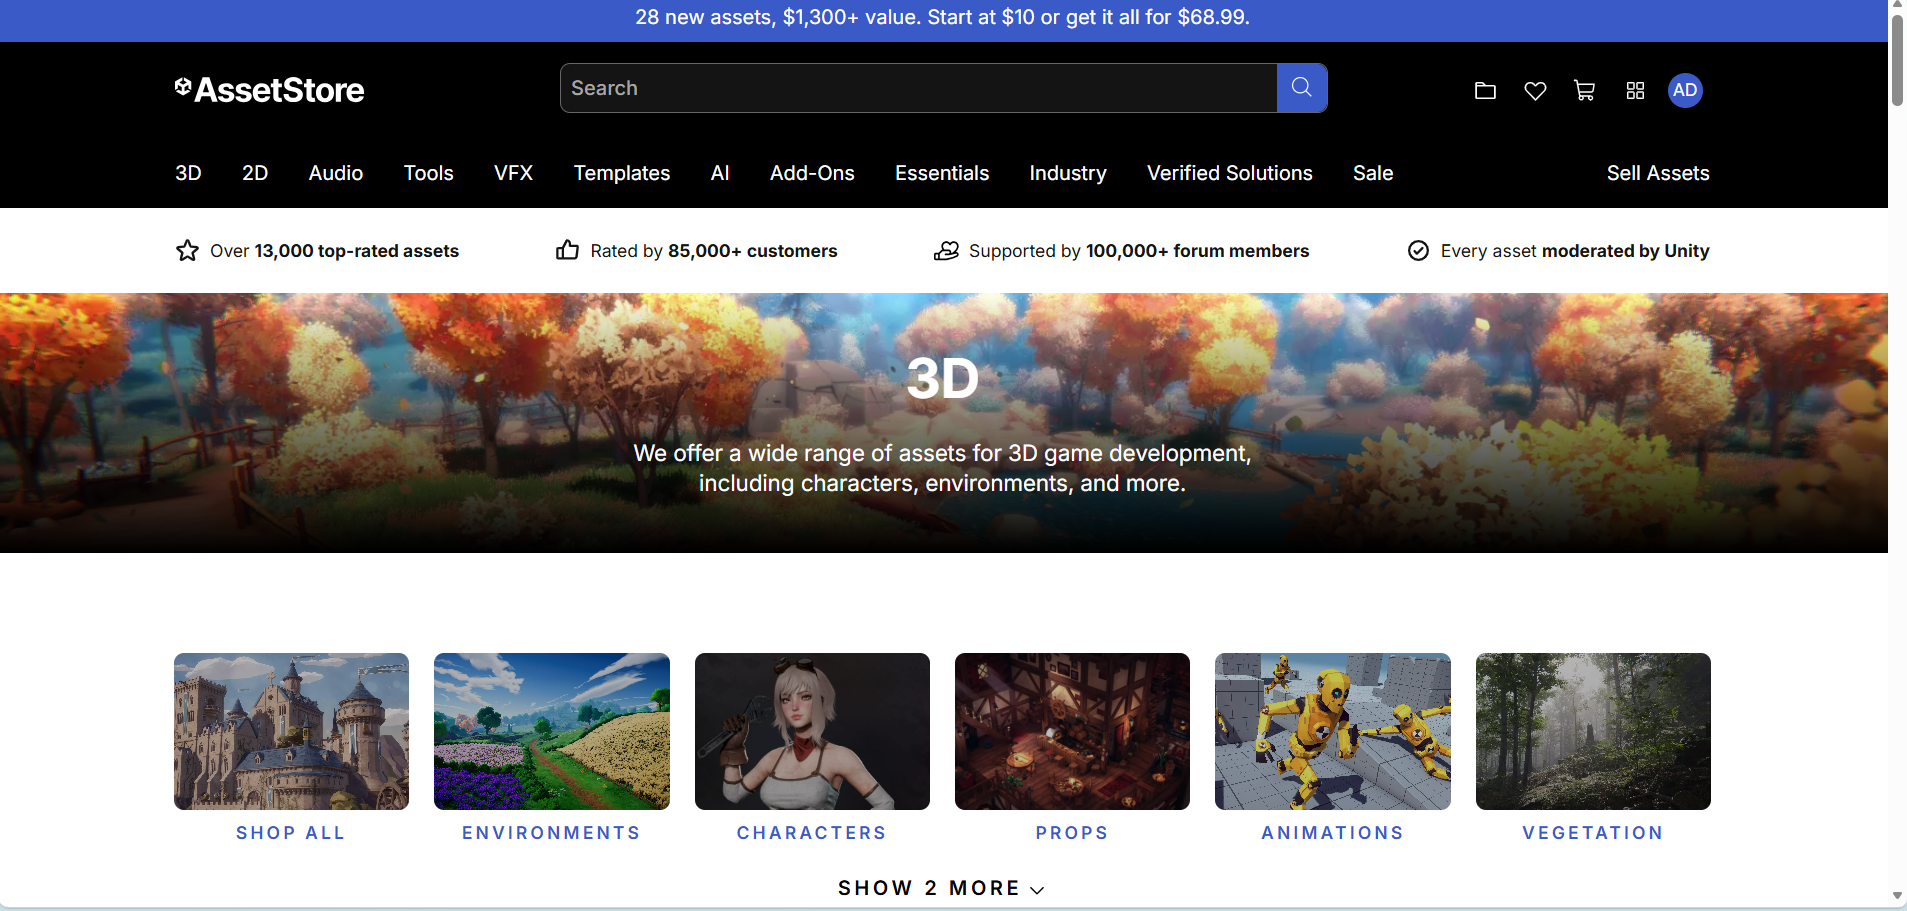
\includegraphics[width=0.5\textwidth]{images/existant/unity.png}
\caption{Unity Asset Store}
\end{figure}

\subsubsection{Fab (Epic Games)}
Fab, Epic Games’ unified marketplace, supports multiple engines and benefits from Unreal Engine integration. Despite its breadth, it lacks customization, internal workflows, and AI-powered features.

\begin{figure}[h]
\centering
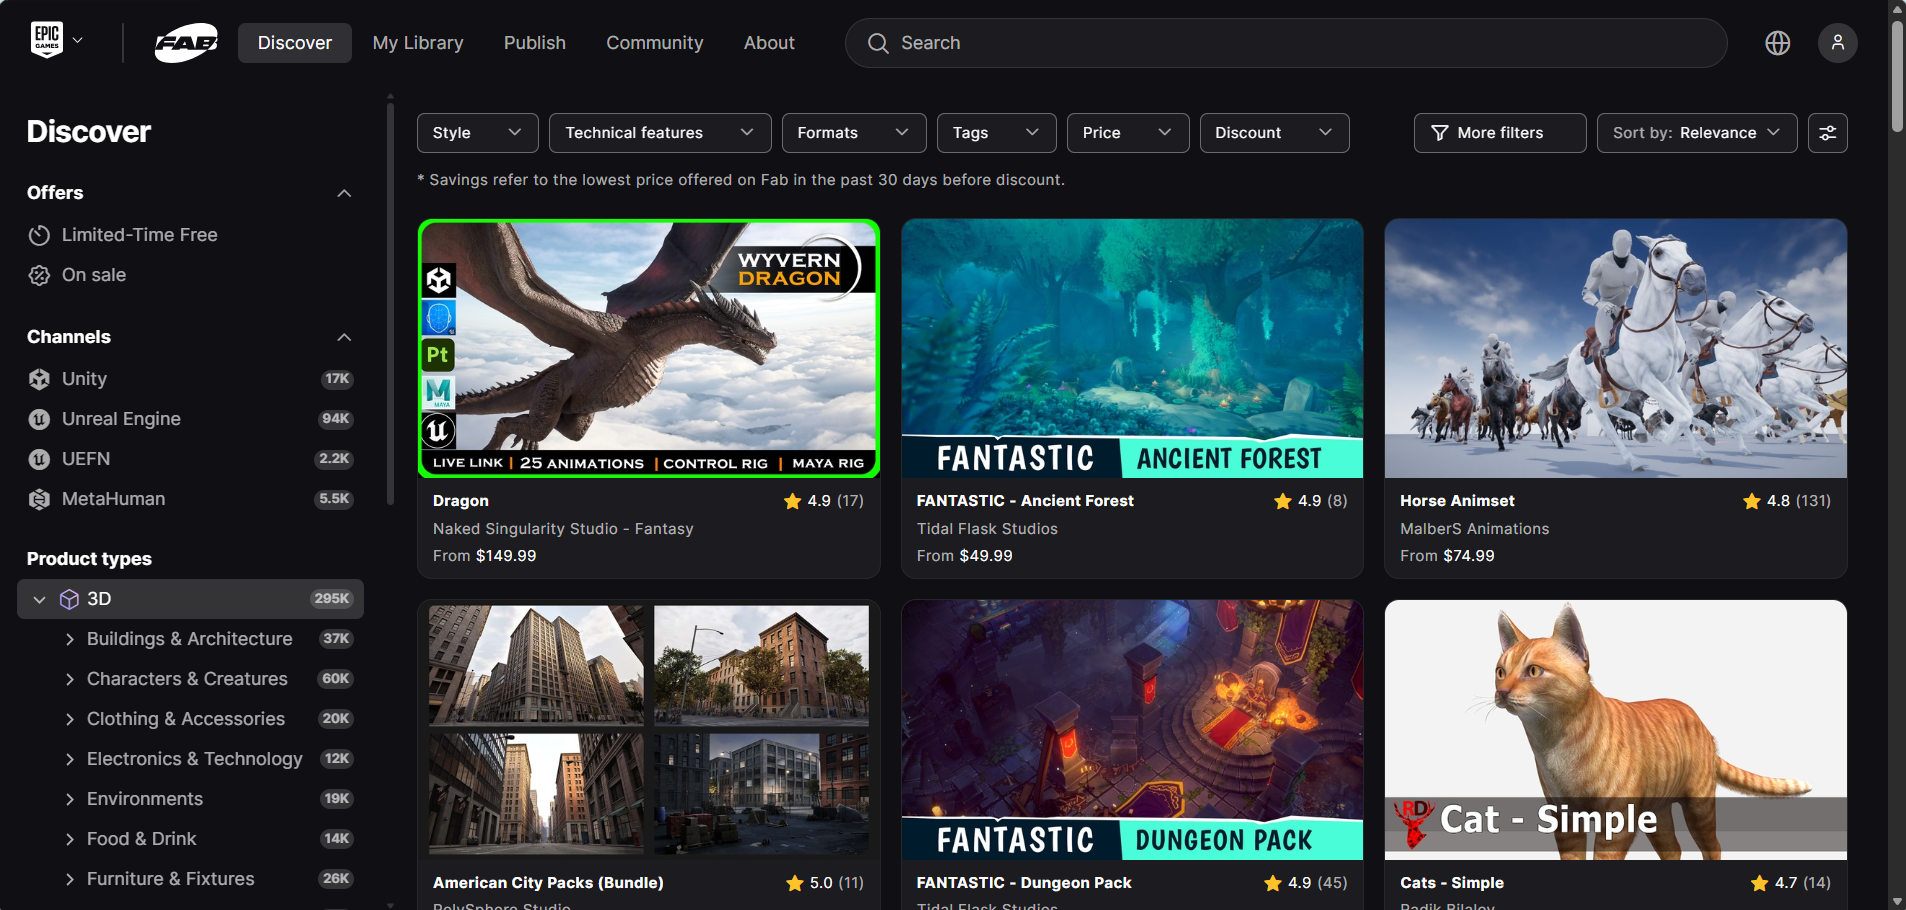
\includegraphics[width=0.5\textwidth]{images/existant/fab.png}
\caption{Fab Marketplace}
\end{figure}

\subsubsection{Sketchfab}
Sketchfab excels in in-browser 3D visualization and supports multiple formats. It is widely used for showcasing models but does not provide monetization flexibility, RBAC, or internal studio management.

\begin{figure}[h]
\centering
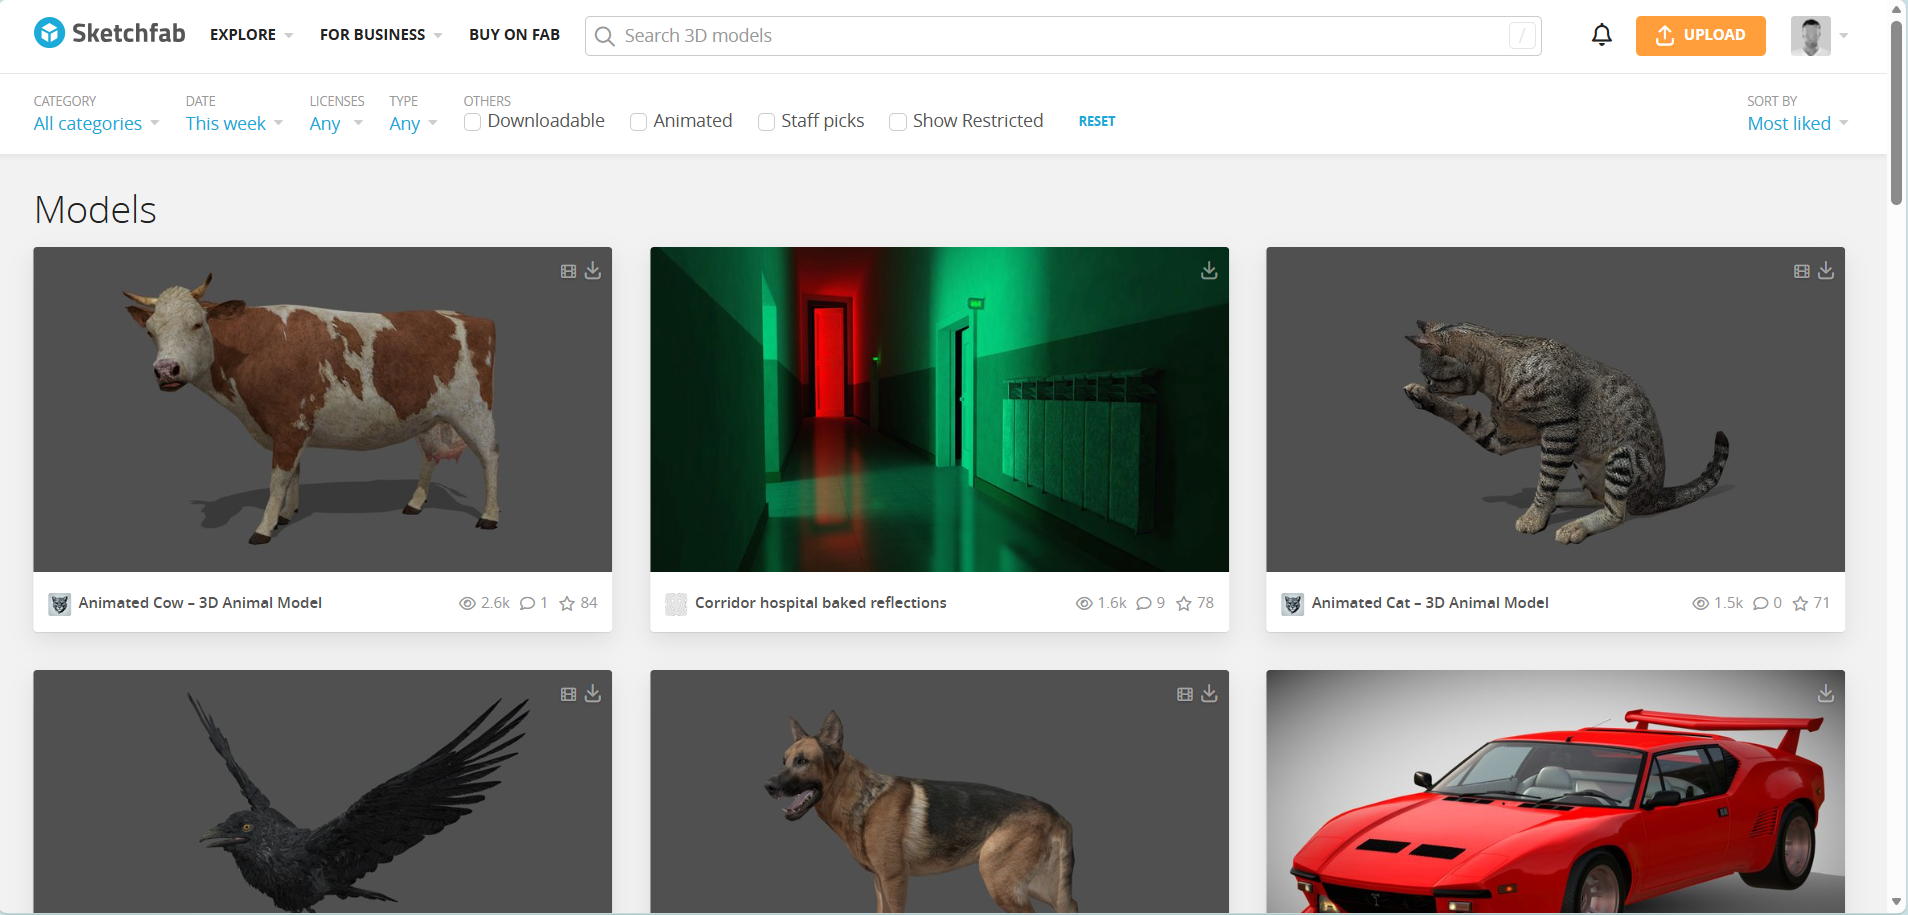
\includegraphics[width=0.5\textwidth]{images/existant/sketchfab.png}
\caption{Sketchfab Platform}
\end{figure}

\subsubsection{CGTrader}
CGTrader offers a large catalog and supports multiple engines. However, it is externally hosted, lacks internal collaboration tools, and does not integrate AI or role-based workflows.

\begin{figure}[h]
\centering
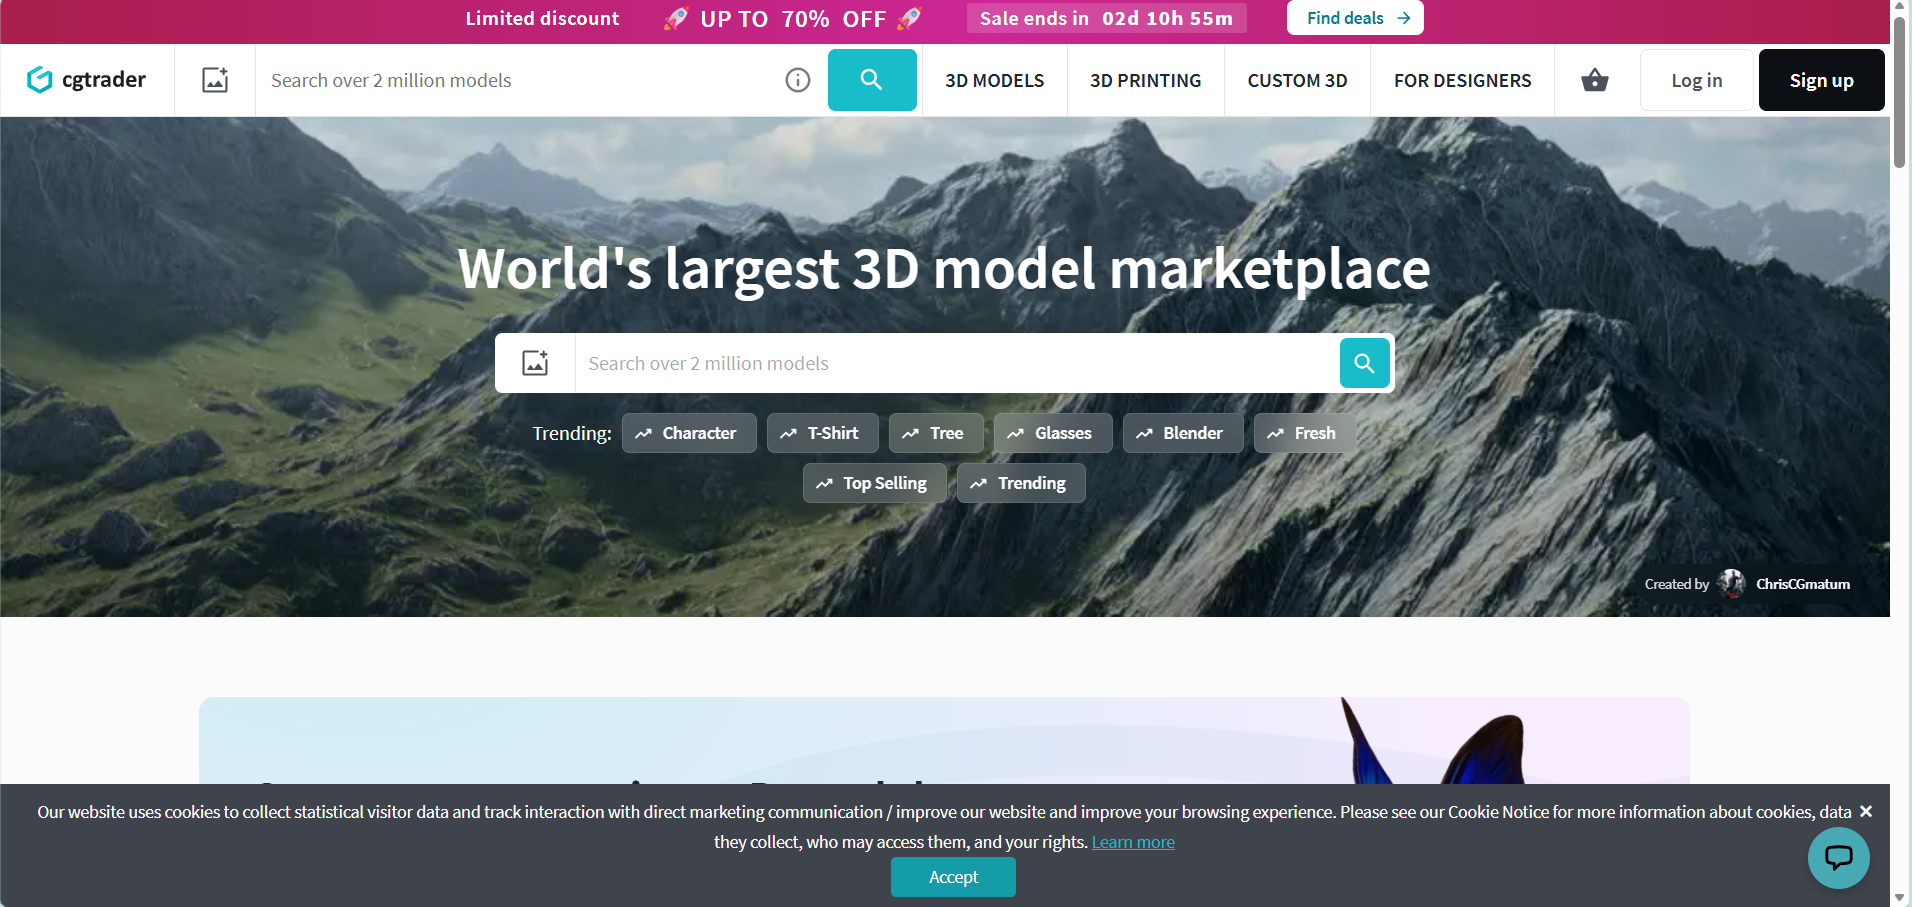
\includegraphics[width=0.5\textwidth]{images/existant/cgtrader.png}
\caption{CGTrader Marketplace}
\end{figure} 

\subsection{Critics}
\begin{itemize}
    \item \textbf{Unity Asset Store}: Limited to Unity, no RBAC, no internal workflows.
    \item \textbf{Fab}: Strong Unreal integration but lacks customization and AI.
    \item \textbf{Sketchfab}: Excellent visualization but weak in monetization and team features.
    \item \textbf{CGTrader}: Large catalog but externally controlled, no studio-oriented tools.
\end{itemize}

None of these platforms combine marketplace features, internal ERP-style modules, RBAC, and AI services in a single self-hosted solution.

\section{Proposed Solution}
The proposed solution is a \textbf{full-stack web platform} composed of two interconnected applications:

\begin{enumerate}
    \item \textbf{IGS Marketplace}: Public-facing marketplace for asset listing, purchase, and moderation. Features include a 3D interactive viewer, Stripe \& Flouci checkout, subscription system, and an AI chatbot assistant.
    \item \textbf{IGS Workspace}: Internal dashboard for employees and interns. Features include task management, project ERP modules, analytics, and real-time chat.
\end{enumerate}

Both applications share the same backend API (Express.js), PostgreSQL database, and JWT authentication, enabling seamless Single Sign-On (SSO).

\subsection{Development Methodology: Scrum}

\textbf{Scrum} was selected as the development methodology because requirements emerged progressively throughout the internship, the company supervisor (Mme. Nour Ltaief) naturally assumes the Product Owner role, the academic supervisor (Mr. Sami Ben Amor) assumes the Scrum Master role, and sprint reviews align with mandatory internship progress meetings.

The project was divided into \textbf{eight sprints}, each lasting approximately two to three weeks:

\begin{table}[H]
\centering
\caption{Sprint Planning Overview}
\begin{tabular}{C{1.2cm} L{4.5cm} L{7.8cm}}
\toprule
\textbf{Sprint} & \textbf{Theme} & \textbf{Key Deliverables} \\
\midrule
0 & Research \& Architecture       & Architecture design, DB schema, environment setup \\
1 & Core Infrastructure            & Backend, PostgreSQL, JWT auth, RBAC (6 roles) \\
2 & Asset Marketplace Core         & Catalog, 3D viewer, seller upload, cart, Stripe \\
3 & Content \& Administration      & Reviews, notifications, admin panel, subscriptions \\
4 & Advanced Role Features         & Intern workflow, seller analytics, trading, groups \\
5 & IGS Workspace                  & Companion app, task management, real-time chat \\
6 & AI Integration                 & ML models, sentiment analysis, chatbot \\
7 \& 8 & AI Expansion \& Polish   & Recommendation engine, UI overhaul, admin dashboard \\
\bottomrule
\end{tabular}
\end{table}

% ---- 1.6 TECHNOLOGY STACK ----
\section{Technology Stack}

\begin{table}[H]
\centering
\caption{Technology Stack Summary}
\begin{tabular}{L{3cm} L{4.5cm} L{6cm}}
\toprule
\textbf{Layer} & \textbf{Technology} & \textbf{Role / Justification} \\
\midrule
\multirow{3}{*}{Frontend}
  & React 18 + Vite           & SPA framework — fast HMR, component model \\
  & Three.js / Model Viewer   & 3D asset viewer in the browser \\
  & TailwindCSS               & Utility-first responsive styling \\
\midrule
\multirow{3}{*}{Backend}
  & Node.js + Express.js      & REST API — non-blocking, JSON-native \\
  & Socket.io                 & WebSocket real-time events (chat, notifications) \\
  & HuggingFace / Mistral-7B  & AI review analysis, chatbot, recommendations \\
\midrule
\multirow{3}{*}{Data \& Auth}
  & PostgreSQL 16             & Primary relational database \\
  & Supabase                  & Scalable file hosting for 3D assets \\
  & Supabase Auth             & Authentication, sessions, and JWT-based access \\
\midrule
Payments & Stripe             & Secure card payment processing \\
\midrule
\multirow{2}{*}{Dev Tools}
  & Git + GitHub              & Version control and CI/CD \\
  & Postman + draw.io         & API testing and UML diagram preparation \\
 
\bottomrule
\end{tabular}
\end{table}

% ---- 1.7 WORK ENVIRONMENT ----
\section{Work Environment}

The project was developed in a modern full-stack environment combining frontend, backend,
database, storage, payment, AI, version-control, and documentation tools. The following
overview summarizes the main tools used during the internship.

\newcommand{\toollogo}[2]{%
\begin{minipage}{0.15\textwidth}
\centering
\includegraphics[height=0.72cm, keepaspectratio]{images/#1}\\[-1pt]
{\scriptsize #2}
\end{minipage}
}

\begin{table}[H]
\centering
\caption{Software Work Environment}
\renewcommand{\arraystretch}{1.35}
\begin{tabularx}{\textwidth}{L{3cm} X}
\toprule
\textbf{Category} & \textbf{Tools} \\
\midrule
Frontend &
\toollogo{logo_react.png}{React}
\toollogo{logo_vite.png}{Vite}
\toollogo{logo_threejs.png}{Three.js}
\toollogo{logo_tailwindcss.png}{TailwindCSS} \\
\midrule
Backend &
\toollogo{logo_nodejs.png}{Node.js}
\toollogo{logo_express.png}{Express.js}
\toollogo{logo_socketio.png}{Socket.io}
\toollogo{logo_jwt.png}{JWT} \\
\midrule
Data, Auth, Storage &
\toollogo{logo_postgresql.png}{PostgreSQL}
\toollogo{logo_supabase.png}{Supabase}
\toollogo{logo_supabase.png}{Supabase Auth}
\toollogo{logo_stripe.png}{Stripe} \\
\midrule
AI and Testing &
\toollogo{logo_huggingface.png}{HuggingFace}
\toollogo{logo_postman.png}{Postman}
\toollogo{logo_eslint.png}{ESLint}
\toollogo{logo_npm.png}{npm} \\
\midrule
DevOps and Documentation &
\toollogo{logo_github.png}{GitHub}
\toollogo{logo_githubactions.png}{Actions}
\toollogo{logo_docker.png}{Docker}
\toollogo{logo_drawio.png}{draw.io} \\
\midrule
Development IDE &
\toollogo{logo_git.png}{Git}
\toollogo{logo_latex.png}{XeLaTeX}
\toollogo{logo_postman.png}{API Tests}
\toollogo{logo_drawio.png}{UML} \\
\bottomrule
\end{tabularx}
\end{table}

\section*{Conclusion}
This chapter established the project context: the host organization IGS and its operational challenges, the comparative analysis confirming the absence of a dedicated 3D marketplace in Tunisia, the proposed two-application solution, the Scrum methodology applied across eight sprints, the technology stack, and the work environment. The following chapter details the functional and non-functional requirements of the system.

% ============================================================
% CHAPTER 2 — REQUIREMENTS ANALYSIS
% ============================================================
\chapter{Requirements Analysis}

\section*{Introduction}
This chapter identifies the system actors, enumerates functional and non-functional requirements, presents the global use case diagram, and defines the system architecture.

% ---- 2.1 ACTORS ----
\section{Actors Identification}

The IGS Marketplace platform serves six distinct actor types organized in a hierarchical RBAC system:

\begin{table}[H]
\centering
\caption{System Actors and Permission Levels}
\begin{tabular}{L{2.5cm} C{2cm} C{2cm} L{7cm}}
\toprule
\textbf{Role}    & \textbf{Type}    & \textbf{Level} & \textbf{Key Permissions} \\
\midrule
super\_admin     & Internal         & 100            & Full system access, manage roles, system settings \\
admin            & Internal         & 80             & Manage users, assets, orders, view analytics \\
employee         & Internal         & 60             & Moderate content, view all analytics \\
intern           & Internal         & 40             & Browse catalog, request free assets, view tasks \\
seller           & External         & 20             & Upload assets, manage own listings, view analytics \\
member           & External         & 10             & Purchase assets, add to cart, write reviews \\
\bottomrule
\end{tabular}
\end{table}

% ---- 2.2 FUNCTIONAL REQUIREMENTS ----
\section{Functional Requirements}

\begin{table}[H]
\centering
\caption{Functional Requirements Summary}
\begin{tabularx}{\textwidth}{L{3.5cm} X}
\toprule
\textbf{Domain} & \textbf{Requirements} \\
\midrule
Authentication       & Register via email/password or Google OAuth2; JWT-based API authentication; profile management; admin role management. \\
\midrule
Asset Catalog        & Browse, filter (category, price, rating, free/paid), and search assets; 13 categories; interactive 3D/HDRI/texture viewer. \\
\midrule
Seller Upload        & Multi-format upload (GLB, FBX, OBJ, PNG, HDR\ldots); pending moderation workflow; edit request after approval; seller analytics dashboard. \\
\midrule
Shopping \& Orders   & Persistent cart; Stripe payment; order tracking; automatic library unlock; free asset claiming. \\
\midrule
Reviews \& Ratings   & Ownership-gated review submission; 1--5 star rating; AI sentiment analysis; automatic moderation flagging. \\
\midrule
Admin Panel          & Approve/reject assets with written reason; manage users and roles; platform-wide analytics; audit trail. \\
\midrule
Notifications        & Real-time and persistent in-app notifications; unread badge; mark as read. \\
\midrule
Intern Workflow      & Asset request with justification; voucher generation; supervised upload. \\
\midrule
Community            & P2P asset trading; community groups; seller role request flow. \\
\midrule
IGS Workspace        & Internal app: team management, task tracking, project ERP, real-time chat (Socket.io), role-based navigation. \\
\midrule
AI Services          & Personalized recommendation engine; marketplace chatbot (Mistral-7B); automated review sentiment analysis. \\
\bottomrule
\end{tabularx}
\end{table}

% ---- 2.3 NON-FUNCTIONAL REQUIREMENTS ----
\section{Non-Functional Requirements}

\begin{table}[H]
\centering
\caption{Non-Functional Requirements}
\begin{tabularx}{\textwidth}{L{3.5cm} X}
\toprule
\textbf{Category}        & \textbf{Requirements} \\
\midrule
\textbf{Performance}     & API response under 300 ms for standard queries; asset files streamed to cloud storage; queries indexed. \\
\textbf{Security}        & JWT expiration; Firebase token verification on all protected routes; RBAC middleware; parameterized queries; CORS; HTTPS in production. \\
\textbf{Scalability}     & Stateless REST API; cloud file storage (Supabase); connection pooling; horizontal scaling ready. \\
\textbf{Usability}       & Responsive UI for desktop and tablet; loading states and error messages on all user-facing operations. \\
\textbf{Reliability}     & Centralized error handling; database transactions for orders; audit logging for admin actions. \\
\textbf{Maintainability} & Routes → Controllers → Repositories separation; modular React components; consistent naming conventions. \\
\bottomrule
\end{tabularx}
\end{table}

% ---- 2.4 GLOBAL USE CASE ----
\section{Global Use Case Diagram}

\begin{figure}[H]
\centering
\resizebox{0.85\textwidth}{!}{% Global Use Case Diagram -- All Actors
\begin{tikzpicture}[
  actor/.style={rectangle, draw=isiBlue, fill=blue!10, rounded corners=3pt,
                minimum width=1.8cm, minimum height=0.65cm, align=center,
                font=\footnotesize\bfseries},
  uc/.style={ellipse, draw=isiBlue!60, fill=blue!4,
             minimum width=3.6cm, minimum height=0.65cm,
             align=center, font=\footnotesize, inner sep=1pt},
  extends/.style={draw=gray, dashed, ->, font=\tiny\itshape},
  assoc/.style={draw=gray!70, thin},
  boundary/.style={draw=isiBlue, very thick, fill=gray!3, rounded corners=6pt}]

  % ---- System Boundary ----
  \draw[boundary] (-4.2,-7.6) rectangle (4.2,5.2);
  \node[font=\footnotesize\bfseries\color{isiBlue}] at (0,5.0) {$\ll$system$\gg$ IGS Marketplace};

  % ---- Use Cases ----
  \node[uc] (browse)      at (0, 4.3)  {Browse Catalog};
  \node[uc] (search)      at (0, 3.4)  {Search \& Filter Assets};
  \node[uc] (viewdetail)  at (0, 2.5)  {View Asset Details (3D)};
  \node[uc] (cart)        at (0, 1.6)  {Manage Cart};
  \node[uc] (purchase)    at (0, 0.7)  {Purchase Asset (Stripe)};
  \node[uc] (download)    at (0,-0.2)  {Download / Library};
  \node[uc] (review)      at (0,-1.1)  {Write Review \& Rate};
  \node[uc] (upload)      at (0,-2.0)  {Upload Asset};
  \node[uc] (analytics)   at (0,-2.9)  {View Analytics};
  \node[uc] (moderate)    at (0,-3.8)  {Moderate Assets};
  \node[uc] (manageusers) at (0,-4.7)  {Manage Users};
  \node[uc] (reqasset)    at (0,-5.6)  {Request Asset (Intern)};
  \node[uc] (voucher)     at (0,-6.5)  {Redeem Voucher};
  \node[uc] (workspace)   at (0,-7.3)  {Access Workspace};

  % ---- Left Actors ----
  \node[actor] (visitor)  at (-7.2, 4.3)  {Visitor};
  \node[actor] (member)   at (-7.2, 1.0)  {Member};
  \node[actor] (seller)   at (-7.2,-2.4)  {Seller};
  \node[actor] (intern)   at (-7.2,-6.0)  {Intern};

  % ---- Right Actors ----
  \node[actor] (admin)    at (7.2,-3.3)   {Admin};
  \node[actor] (superadm) at (7.2,-6.5)   {Super Admin};
  \node[actor] (employee) at (7.2,-0.2)   {Employee};

  % ---- Associations ----
  % Visitor
  \draw[assoc] (visitor) -- (browse);
  \draw[assoc] (visitor) -- (search);
  \draw[assoc] (visitor) -- (viewdetail);

  % Member (inherits visitor)
  \draw[assoc] (member) -- (browse);
  \draw[assoc] (member) -- (cart);
  \draw[assoc] (member) -- (purchase);
  \draw[assoc] (member) -- (download);
  \draw[assoc] (member) -- (review);

  % Seller
  \draw[assoc] (seller) -- (upload);
  \draw[assoc] (seller) -- (analytics);
  \draw[assoc] (seller) -- (download);

  % Intern
  \draw[assoc] (intern) -- (browse);
  \draw[assoc] (intern) -- (reqasset);
  \draw[assoc] (intern) -- (voucher);
  \draw[assoc] (intern) -- (workspace);

  % Admin
  \draw[assoc] (admin) -- (moderate);
  \draw[assoc] (admin) -- (manageusers);
  \draw[assoc] (admin) -- (analytics);

  % Employee
  \draw[assoc] (employee) -- (moderate);
  \draw[assoc] (employee) -- (workspace);

  % Super Admin (extends Admin)
  \draw[assoc] (superadm) -- (manageusers);
  \draw[assoc] (superadm) -- (moderate);
  \draw[extends] (superadm) -- node[right, font=\tiny] {$\ll$extends$\gg$} (admin);

\end{tikzpicture}
}
\caption{Global Use Case Diagram}
\label{fig:use_case_global}
\end{figure}

% ---- 2.5 SYSTEM ARCHITECTURE ----
\section{System Architecture}

The IGS platform follows a \textbf{three-tier distributed architecture} separating presentation, business logic, and data access:

\begin{itemize}
  \item \textbf{Tier 1 — Presentation:} Two independent React + Vite SPAs (Marketplace on port 5173 and IGS Workspace on port 5174), communicating with the backend exclusively via REST and sharing a JWT stored in \texttt{localStorage}.
  \item \textbf{Tier 2 — Business Logic:} A single Express.js REST API (port 3001) handling authentication, authorization, domain logic, and external service orchestration (Stripe, Supabase, Firebase, AI).
  \item \textbf{Tier 3 — Data:} A PostgreSQL database (30+ tables) for relational persistence, and Supabase Storage for binary asset files.
\end{itemize}

Within Tier 2, the backend follows the \textbf{Repository pattern} — each entity has its own repository file encapsulating all SQL queries. Controllers never write raw SQL; they always go through a repository method. This decouples business logic from database access and makes the data layer independently testable.

\begin{figure}[H]
\centering
\resizebox{\textwidth}{!}{% Backend Layered Architecture (3-Tier + Repository Pattern)
\begin{tikzpicture}[
  layer/.style={rectangle, draw=isiBlue, fill=blue!6, rounded corners=4pt,
                minimum width=10cm, minimum height=1.1cm, align=center,
                font=\small\bfseries, text=isiBlue},
  module/.style={rectangle, draw=igsGreen!80, fill=green!5, rounded corners=3pt,
                 minimum width=2.6cm, minimum height=0.85cm, align=center,
                 font=\footnotesize, text=black},
  cross/.style={rectangle, draw=orange!80, fill=orange!8, rounded corners=3pt,
                minimum width=2.2cm, minimum height=0.75cm, align=center,
                font=\footnotesize, text=black},
  arr/.style={->, thick, draw=isiBlue},
  lbl/.style={font=\tiny\itshape, midway, left}]

  % ── Tier 1 : Presentation / Route Layer ──────────────────────────
  \node[layer] (routes) at (0, 6) {Tier 1 — Presentation / API Routes Layer};
  \node[module] at (-3.5, 5.1) {\texttt{routes/auth.js}};
  \node[module] at (-1.1, 5.1) {\texttt{routes/assets.js}};
  \node[module] at (1.3,  5.1) {\texttt{routes/orders.js}};
  \node[module] at (3.7,  5.1) {\texttt{routes/users.js}};

  % ── Middleware band ───────────────────────────────────────────────
  \node[draw=darkGray, fill=gray!8, rounded corners=3pt,
        minimum width=10cm, minimum height=0.65cm, align=center,
        font=\footnotesize\itshape, text=darkGray] at (0, 4.3)
        {Middleware: \texttt{authenticate} · \texttt{requirePermission} · \texttt{rateLimiter} · \texttt{errorHandler}};

  % ── Tier 2 : Business Logic / Controller Layer ────────────────────
  \node[layer] (controllers) at (0, 3.5) {Tier 2 — Business Logic / Controller Layer};
  \node[module] at (-3.5, 2.6) {\texttt{authController}};
  \node[module] at (-1.1, 2.6) {\texttt{assetController}};
  \node[module] at (1.3,  2.6) {\texttt{orderController}};
  \node[module] at (3.7,  2.6) {\texttt{userController}};

  % ── Tier 3 : Data Access / Repository Layer ───────────────────────
  \node[layer] (repos) at (0, 1.8) {Tier 3 — Data Access / Repository Layer};
  \node[module] at (-3.5, 0.9) {\texttt{userRepository}};
  \node[module] at (-1.1, 0.9) {\texttt{assetRepository}};
  \node[module] at (1.3,  0.9) {\texttt{orderRepository}};
  \node[module] at (3.7,  0.9) {\texttt{cartRepository}};

  % ── Database ──────────────────────────────────────────────────────
  \node[cylinder, draw=darkGray, fill=gray!12, shape border rotate=90,
        minimum width=4cm, minimum height=0.9cm, align=center,
        font=\footnotesize\bfseries] at (0, 0) {PostgreSQL Database};

  % ── Cross-cutting Services ────────────────────────────────────────
  \node[font=\footnotesize\bfseries\color{orange!80!black}]
        at (6.7, 3.5) {Cross-cutting};
  \node[cross] at (6.7, 2.9) {\texttt{storageService}};
  \node[cross] at (6.7, 2.0) {\texttt{auditService}};
  \node[cross] at (6.7, 1.1) {\texttt{aiService}};
  \node[cross] at (6.7, 0.2) {\texttt{tokenBlacklist}};

  % ── Arrows between tiers ─────────────────────────────────────────
  \draw[arr] (routes) -- node[lbl] {delegates} (controllers);
  \draw[arr] (controllers) -- node[lbl] {queries} (repos);
  \draw[arr] (repos.south) -- node[lbl] {SQL} (0, 0.45);

\end{tikzpicture}
}
\caption{Backend Layered Architecture --- Routes → Controllers → Repositories}
\label{fig:arch_backend}
\end{figure}

\section*{Conclusion}
This chapter identified all system actors, detailed functional and non-functional requirements, and established the architectural foundation. The platform follows a three-tier distributed architecture with the Repository pattern on the backend. The following chapters each cover one sprint or pair of sprints of the development cycle.

% ============================================================
% CHAPTER 3 -- STUDY AND IMPLEMENTATION OF SPRINT 1 AND SPRINT 2
% ============================================================
\chapter{Marketplace Foundations}
\label{chap:sprints12}
\chaptersommaire
\clearpage

\chapterintro{%
This chapter presents the study and implementation of Sprint~1 and Sprint~2, covering the authentication and access-control foundation, followed by the public marketplace experience.%
}

% ============================================================
% SPRINT 1 — AUTHENTICATION & RBAC
% ============================================================
\section{Sprint 1: Authentication, Profiles and RBAC}

Sprint~1 builds the access foundation. It covers user registration, sign-in, password
recovery, profile management and the role-based access control model on which every
subsequent feature relies.

\subsection{Sprint 1 Backlog}

Table~\ref{tab:sprint1_backlog} summarizes the backlog of the first sprint.

\begin{table}[H]
\centering
\caption{Sprint 1 Backlog}
\renewcommand{\arraystretch}{1.2}
\begin{tabular}{|C{0.6cm}|L{10cm}|C{2.5cm}|}
\hline
\rowcolor{isiBlue}
\textcolor{white}{\textbf{ID}} &
\textcolor{white}{\textbf{User Story}} &
\textcolor{white}{\textbf{Estimation}} \\
\hline
1 & As a visitor, I want to create an account using email/password or OAuth so I can access protected features. & 4 days \\
\hline
2 & As a registered user, I want to sign in and receive a JWT so I can call protected endpoints. & 3 days \\
\hline
3 & As a user, I want to reset my password by email so I can recover my account. & 2 days \\
\hline
4 & As a user, I want to manage my profile so my public page stays up to date. & 2 days \\
\hline
5 & As an administrator, I want each user to belong to a role that grants a specific set of permissions. & 3 days \\
\hline
6 & As an administrator, I want sensitive actions to be logged. & 2 days \\
\hline
\end{tabular}
\label{tab:sprint1_backlog}
\end{table}

\subsection{Sprint 1 Conception}

\subsubsection{Use Case Diagram}

The figure below illustrates the use case diagram relative to Sprint~1.

\begin{figure}[H]
\centering
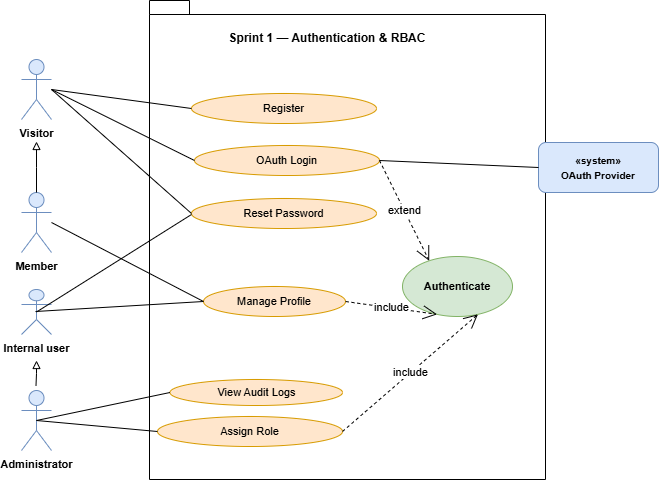
\includegraphics[width=0.9\textwidth]{images/diagrams/uc_s1.png}
\caption{Use case diagram --- Sprint 1}
\label{fig:uc_sprint1}
\end{figure}

\paragraph{Textual description of the use case «Authenticate».}

\begin{table}[H]
\centering
\caption{Use case description: Authenticate}
\label{tab:uc_authenticate}
\renewcommand{\arraystretch}{1.3}
\begin{tabularx}{\textwidth}{|L{3.2cm}|X|}
\hline
\textbf{Use case} & Authenticate \\
\hline
\textbf{Actor} & Registered user \\
\hline
\textbf{Pre-condition} & The user has an active account. \\
\hline
\textbf{Post-condition} & The user holds a valid JWT and can access protected routes. \\
\hline
\textbf{Nominal scenario} &
1. The user opens the sign-in page. \newline
2. The user enters email and password. \newline
3. The system verifies the credentials. \newline
4. The system signs a JWT and returns it to the browser. \newline
5. The browser stores the token and redirects to the marketplace. \\
\hline
\textbf{Alternative scenario} &
3.1. If the credentials are invalid, the system returns an error message. \newline
3.2. Resume at step 2.
\\
\hline
\end{tabularx}
\end{table}

\paragraph{Textual description of the use case «Reset Password».}

\begin{table}[H]
\centering
\caption{Use case description: Reset Password}
\label{tab:uc_reset}
\renewcommand{\arraystretch}{1.3}
\begin{tabularx}{\textwidth}{|L{3.2cm}|X|}
\hline
\textbf{Use case} & Reset Password \\
\hline
\textbf{Actor} & Registered user \\
\hline
\textbf{Pre-condition} & The user has lost access to the account but knows the email. \\
\hline
\textbf{Post-condition} & The password is updated and the user can sign in again. \\
\hline
\textbf{Nominal scenario} &
1. The user requests a reset link by entering an email. \newline
2. The system generates a reset token and emails the reset link. \newline
3. The user opens the link and submits a new password. \newline
4. The system validates the token and stores the new hashed password. \newline
5. A confirmation message is displayed. \\
\hline
\textbf{Alternative scenario} &
4.1. If the token is expired or invalid, an error message is shown. \newline
4.2. The user requests a new reset link.
\\
\hline
\end{tabularx}
\end{table}

\paragraph{Textual description of the use case «Assign Role».}

\begin{table}[H]
\centering
\caption{Use case description: Assign Role}
\label{tab:uc_assign_role}
\renewcommand{\arraystretch}{1.3}
\begin{tabularx}{\textwidth}{|L{3.2cm}|X|}
\hline
\textbf{Use case} & Assign Role \\
\hline
\textbf{Actor} & Administrator \\
\hline
\textbf{Pre-condition} & The administrator is authenticated. \\
\hline
\textbf{Post-condition} & The target user has the chosen role and the associated permissions. \\
\hline
\textbf{Nominal scenario} &
1. The administrator opens the user management page. \newline
2. The administrator selects a user. \newline
3. The administrator chooses a role from the list. \newline
4. The system updates the role assignment and logs the action. \newline
5. A success message is displayed. \\
\hline
\textbf{Alternative scenario} &
3.1. If the administrator does not have the permission to assign the chosen role, an error is shown. \newline
3.2. The administrator picks a different role.
\\
\hline
\end{tabularx}
\end{table}

\subsubsection{Sequence Diagrams}

\paragraph{Sequence diagram «Authenticate».}
When a user attempts to authenticate, the browser sends the credentials to the
\texttt{AuthController}. The system looks up the user record, verifies the password
hash and signs a JWT. The token is returned to the browser, which stores it and
attaches it as a Bearer header on every subsequent call. If credentials are invalid,
the system returns an error and no token is issued.

\begin{figure}[H]
\centering
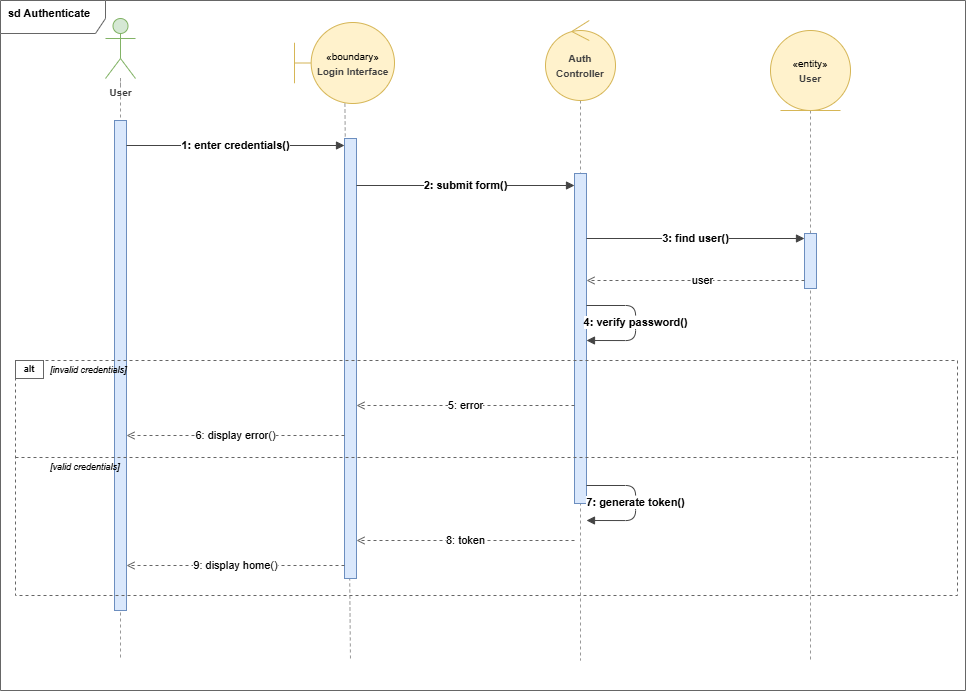
\includegraphics[width=\textwidth]{images/diagrams/seq_auth.png}
\caption{Sequence diagram «Authenticate»}
\label{fig:seq_auth}
\end{figure}

\paragraph{Sequence diagram «Reset Password».}
When a user requests a password reset, the system generates a unique token, stores it
on the user record with an expiry, and sends a reset link by email. When the user
opens the link and submits a new password, the system verifies the token, hashes the
new password and clears the reset token. If the token is missing or expired, the
system rejects the request.

\begin{figure}[H]
\centering
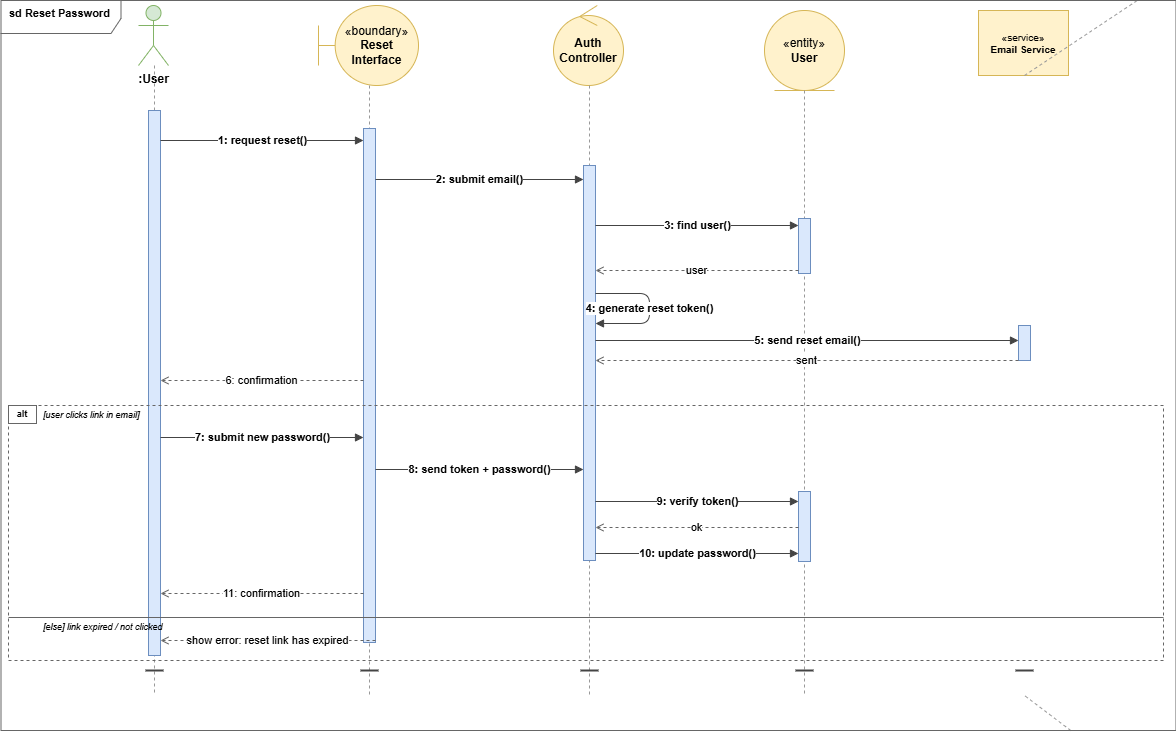
\includegraphics[width=\textwidth]{images/diagrams/seq_reset.png}
\caption{Sequence diagram «Reset Password»}
\label{fig:seq_reset}
\end{figure}

\subsubsection{Class Diagram}

The class diagram of Sprint~1 centres on the \texttt{User} entity linked to the RBAC
trio \texttt{Role}, \texttt{Permission} and \texttt{AuditLog}. A user holds one or
more roles, each role carries a set of permissions, and every sensitive action is
traced in the audit log.

\begin{figure}[H]
\centering
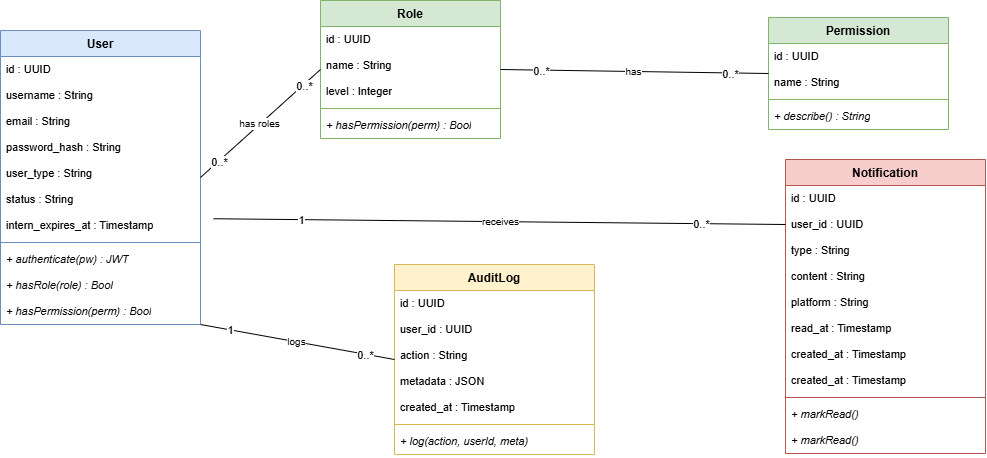
\includegraphics[width=0.95\textwidth]{images/diagrams/class_s1.png}
\caption{Class diagram --- Sprint 1}
\label{fig:class_s1}
\end{figure}

\subsection{Sprint 1 Realization}

In this section we present the interfaces developed during Sprint~1.

\paragraph{«Sign-in interface».}
This interface allows the user to authenticate securely through email and password or
through an OAuth provider. On success, the system stores the JWT and redirects to the
marketplace.

\begin{figure}[H]
\centering
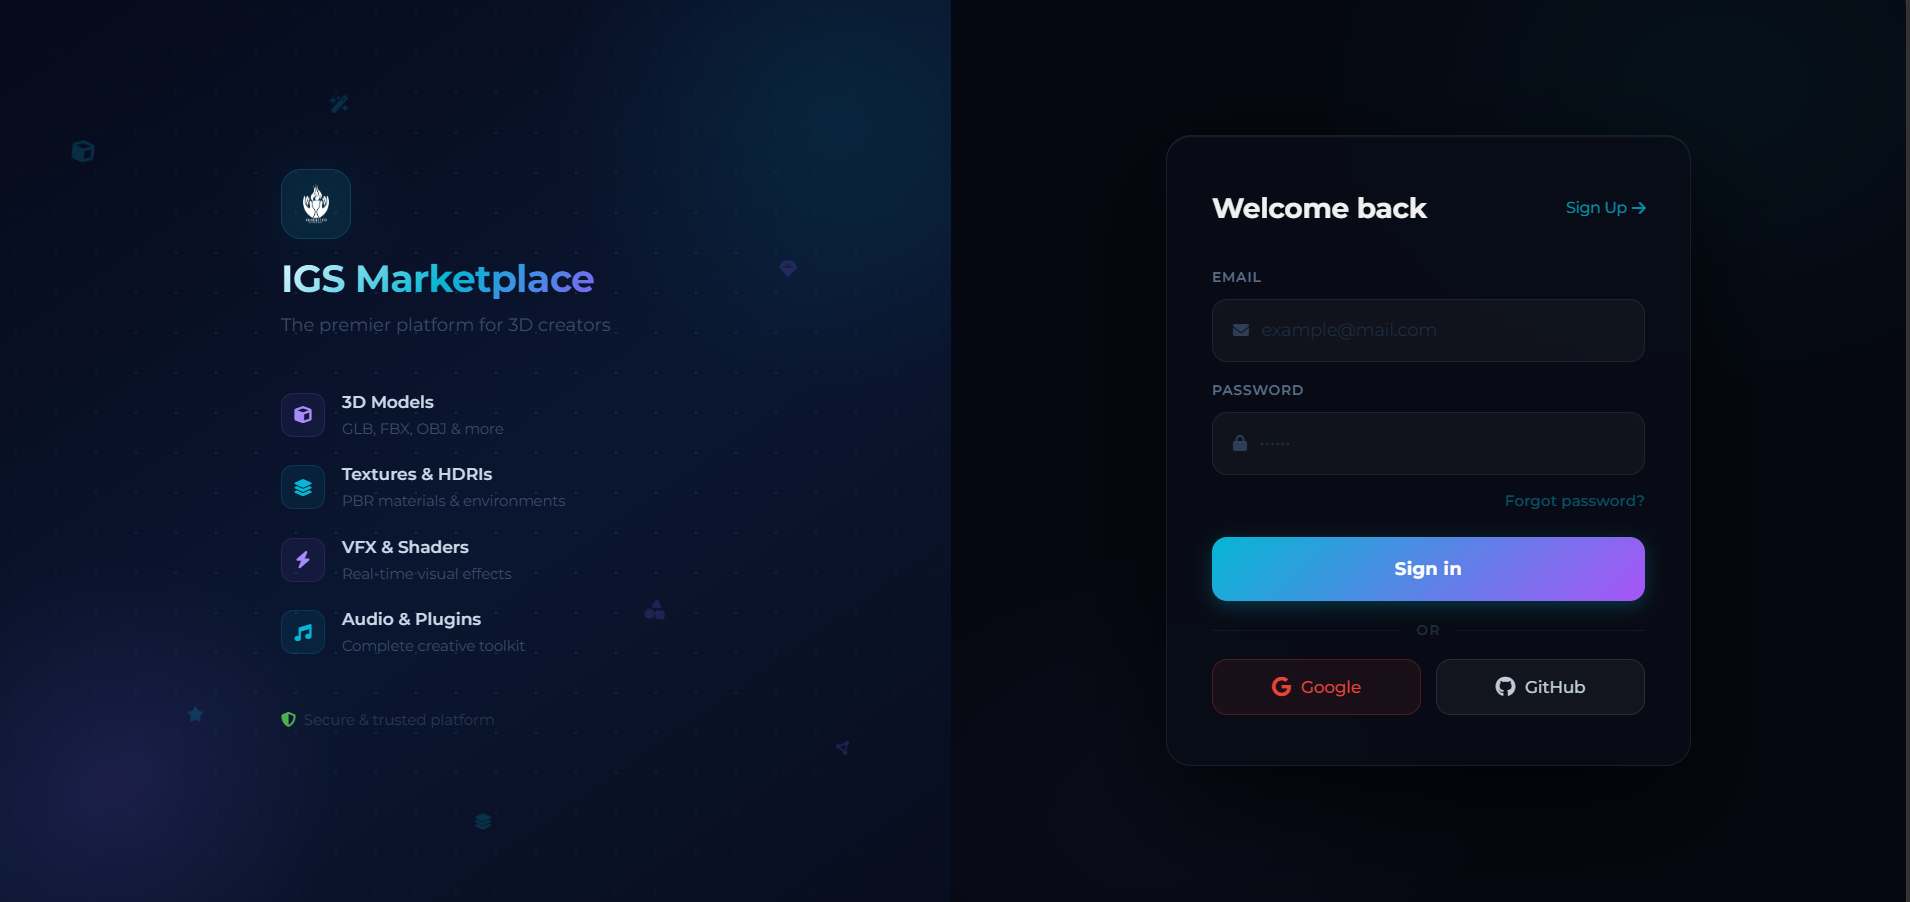
\includegraphics[width=0.8\textwidth]{images/realisation/marketplace/login.png}
\caption{Interface «Sign in»}
\end{figure}

\paragraph{«Sign-up interface».}
This interface lets a new visitor create an account by filling in a short form.
Validation is enforced on the email format and the password strength.

\begin{figure}[H]
\centering
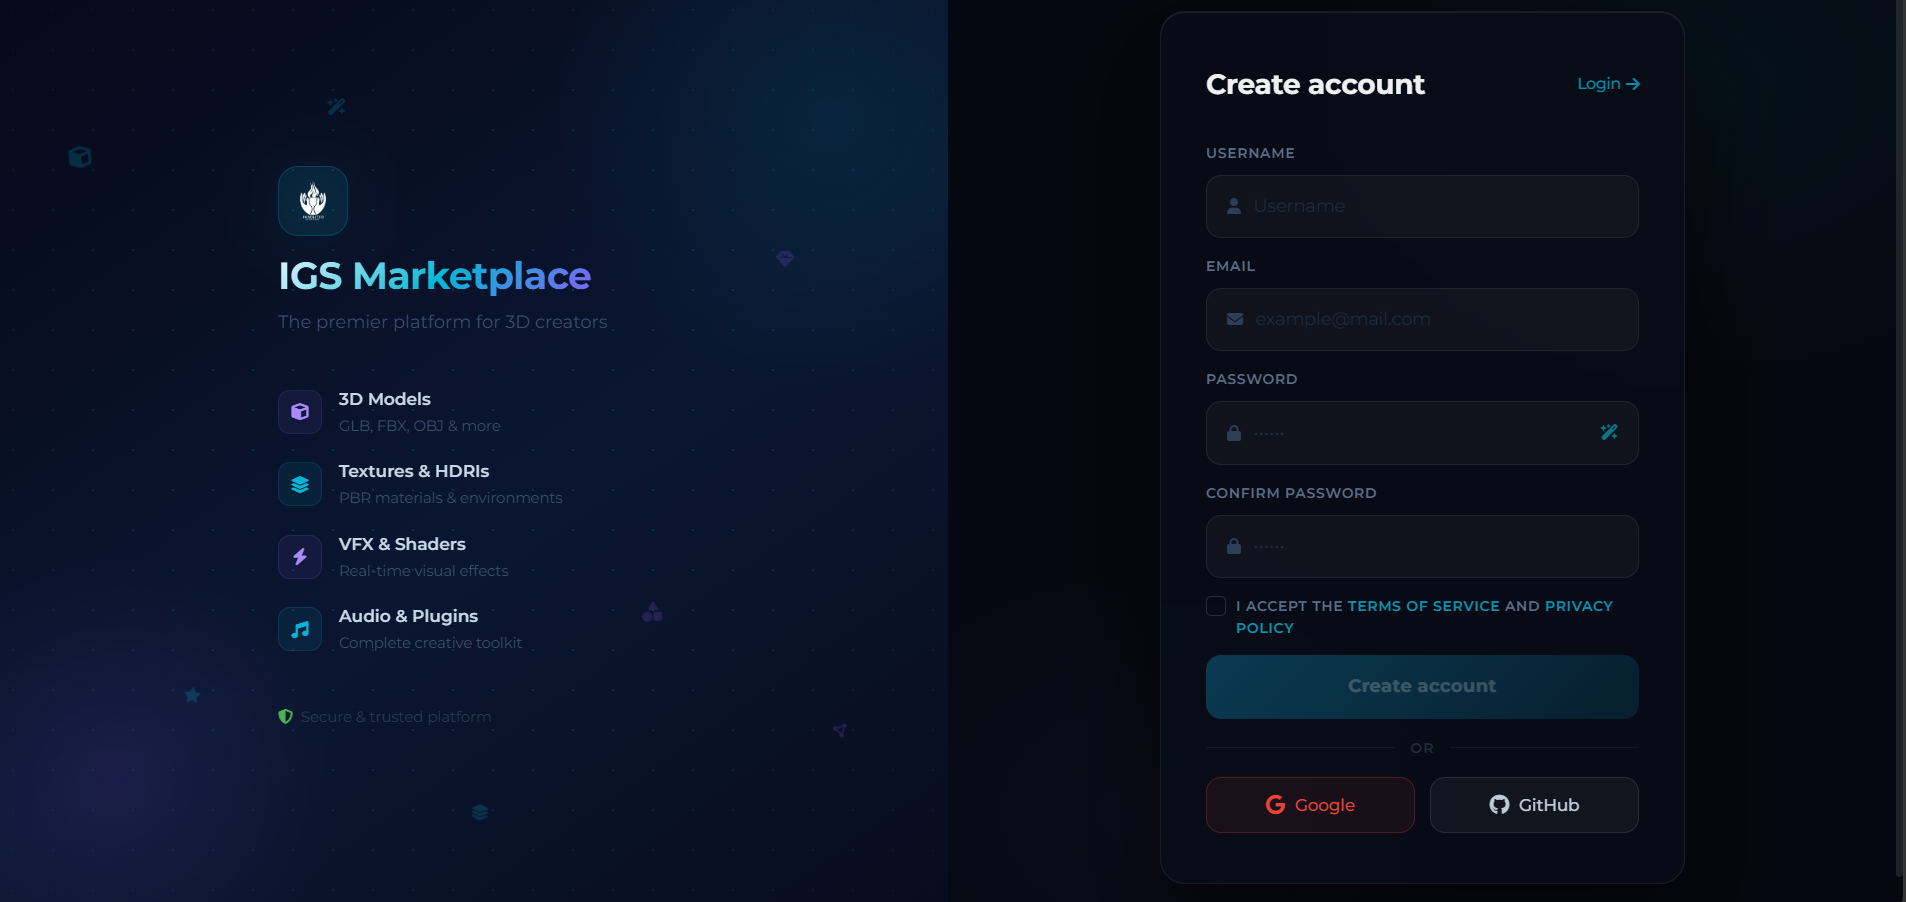
\includegraphics[width=0.8\textwidth]{images/realisation/marketplace/signup.png}
\caption{Interface «Sign up»}
\end{figure}

\paragraph{«Profile management».}
This interface allows the authenticated user to view and update personal information
(avatar, display name, bio, contact details) and to change the account password.

\begin{figure}[H]
\centering
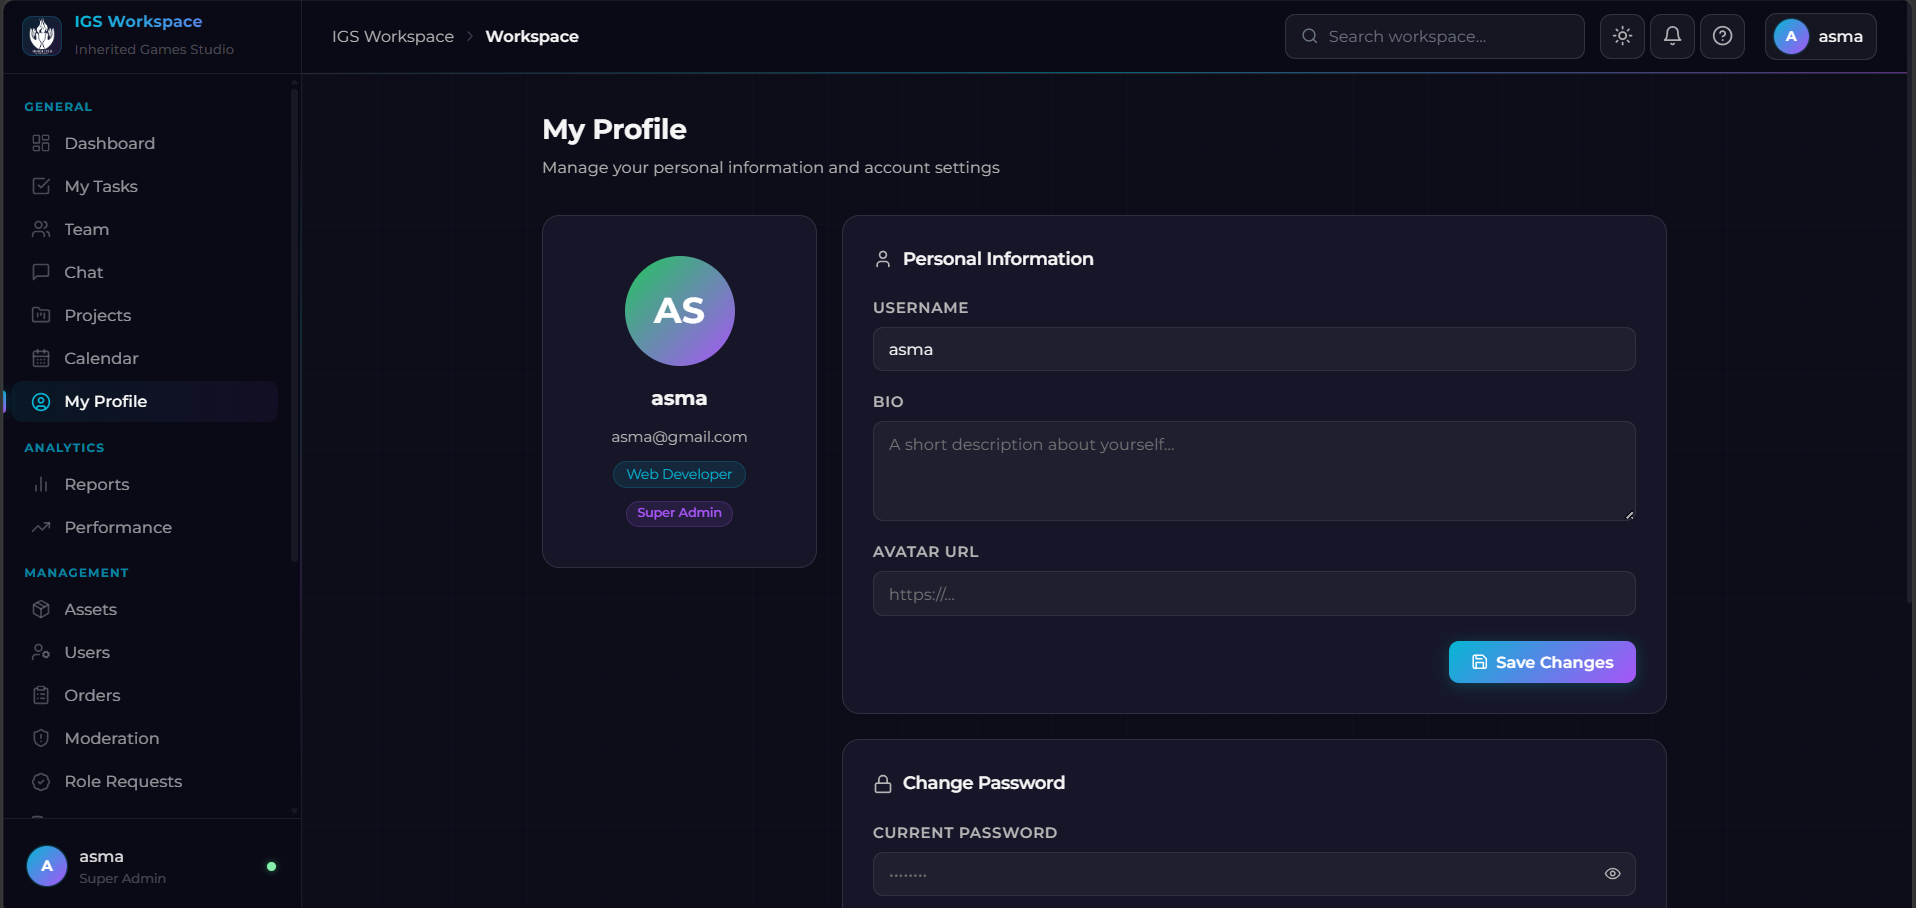
\includegraphics[width=0.8\textwidth]{images/realisation/marketplace/profile.png}
\caption{Interface «Profile»}
\end{figure}

\subsection{Sprint 1 Conclusion}
At the end of Sprint~1 the platform has a working authentication layer with JWT and
OAuth, a profile management page, and a hierarchical RBAC model with six roles. This
foundation conditions every feature delivered in the following sprints.

% ============================================================
% SPRINT 2 — MARKETPLACE CATALOG, PAYMENT, LIBRARY
% ============================================================
\section{Sprint 2: Catalog, Cart, Payment and Library}

Sprint~2 turns the platform into a usable storefront. It delivers the filterable asset
catalog, the interactive 3D and WebXR previews, the shopping cart, the Stripe and
Flouci payment flows and the personal download library.

\subsection{Sprint 2 Backlog}

Table~\ref{tab:sprint2_backlog} summarizes the backlog of the second sprint.

\begin{table}[H]
\centering
\caption{Sprint 2 Backlog}
\renewcommand{\arraystretch}{1.2}
\begin{tabular}{|C{0.6cm}|L{10cm}|C{2.5cm}|}
\hline
\rowcolor{isiBlue}
\textcolor{white}{\textbf{ID}} &
\textcolor{white}{\textbf{User Story}} &
\textcolor{white}{\textbf{Estimation}} \\
\hline
1 & As a visitor, I want to browse a paginated catalogue with filters by category, price and tags. & 3 days \\
\hline
2 & As a visitor, I want to consult an asset detail page with a 3D preview adapted to the asset type. & 4 days \\
\hline
3 & As a member, I want to enter VR / immersive mode for compatible 3D assets so I can inspect them at scale. & 2 days \\
\hline
4 & As a member, I want to add or remove assets from a personal cart. & 2 days \\
\hline
5 & As a member, I want to pay for the cart through Stripe or Flouci and receive instant access. & 4 days \\
\hline
6 & As a member, I want a personal library listing all the assets I can download, with signed-URL downloads. & 3 days \\
\hline
\end{tabular}
\label{tab:sprint2_backlog}
\end{table}

\subsection{Sprint 2 Conception}

\subsubsection{Use Case Diagram}

The figure below illustrates the use case diagram relative to Sprint~2.

\begin{figure}[H]
\centering
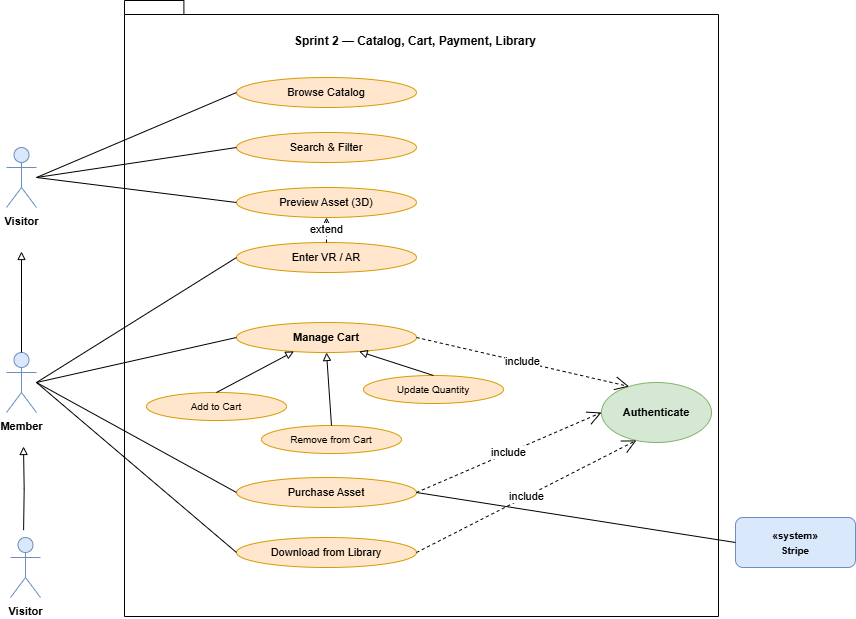
\includegraphics[width=0.9\textwidth]{images/diagrams/uc_s2.png}
\caption{Use case diagram --- Sprint 2}
\label{fig:uc_sprint2}
\end{figure}

\paragraph{Textual description of the use case «Browse and Filter Catalog».}

\begin{table}[H]
\centering
\caption{Use case description: Browse and Filter Catalog}
\label{tab:uc_browse}
\renewcommand{\arraystretch}{1.3}
\begin{tabularx}{\textwidth}{|L{3.2cm}|X|}
\hline
\textbf{Use case} & Browse and Filter Catalog \\
\hline
\textbf{Actor} & Visitor / Member \\
\hline
\textbf{Pre-condition} & The catalog page is accessible. \\
\hline
\textbf{Post-condition} & The catalog displays the filtered list of approved assets. \\
\hline
\textbf{Nominal scenario} &
1. The visitor opens a category page. \newline
2. The visitor applies filters on price, rating or tags. \newline
3. The system queries the catalog with the selected filters. \newline
4. The system returns a paginated list of matching assets. \newline
5. The visitor clicks an asset card to open the detail page. \\
\hline
\textbf{Alternative scenario} &
4.1. If no asset matches the filters, an empty-state message is displayed. \\
\hline
\end{tabularx}
\end{table}

\paragraph{Textual description of the use case «Purchase an Asset».}

\begin{table}[H]
\centering
\caption{Use case description: Purchase an Asset}
\label{tab:uc_purchase}
\renewcommand{\arraystretch}{1.3}
\begin{tabularx}{\textwidth}{|L{3.2cm}|X|}
\hline
\textbf{Use case} & Purchase an Asset \\
\hline
\textbf{Actor} & Member \\
\hline
\textbf{Pre-condition} & The member is authenticated and has at least one asset in the cart. \\
\hline
\textbf{Post-condition} & The order is recorded as paid and the asset is available in the library. \\
\hline
\textbf{Nominal scenario} &
1. The member opens the cart and clicks Checkout. \newline
2. The member selects Stripe or Flouci as payment method. \newline
3. The system creates a payment intent and presents the card form. \newline
4. The payment gateway confirms the transaction. \newline
5. The system records the order, copies the cart items and unlocks the library. \newline
6. A confirmation message is shown. \\
\hline
\textbf{Alternative scenario} &
4.1. If the payment fails, the order stays pending and the library is not unlocked. \newline
4.2. The member can retry from the cart. \\
\hline
\end{tabularx}
\end{table}

\paragraph{Textual description of the use case «Download from Library».}

\begin{table}[H]
\centering
\caption{Use case description: Download from Library}
\label{tab:uc_download}
\renewcommand{\arraystretch}{1.3}
\begin{tabularx}{\textwidth}{|L{3.2cm}|X|}
\hline
\textbf{Use case} & Download from Library \\
\hline
\textbf{Actor} & Member \\
\hline
\textbf{Pre-condition} & The member has at least one asset unlocked in the library. \\
\hline
\textbf{Post-condition} & The asset file is downloaded to the user's machine. \\
\hline
\textbf{Nominal scenario} &
1. The member opens the library page. \newline
2. The member clicks Download on an asset. \newline
3. The system re-checks the access level for the asset. \newline
4. The system generates a signed URL with a one-hour validity. \newline
5. The browser fetches the file directly from cloud storage. \\
\hline
\textbf{Alternative scenario} &
3.1. If the access level is blocked, the system returns a 403 error. \\
\hline
\end{tabularx}
\end{table}

\subsubsection{Sequence Diagrams}

\paragraph{Sequence diagram «Purchase an Asset».}
When a member proceeds to checkout, the backend creates a payment intent at the
gateway and returns the client secret to the browser. The user confirms the card and
the gateway notifies the backend of success. The backend then opens a transaction,
inserts the order, copies the cart items into \texttt{order\_items} with the locked
commission split, grants library access, and returns the confirmation to the browser.

\begin{figure}[H]
\centering
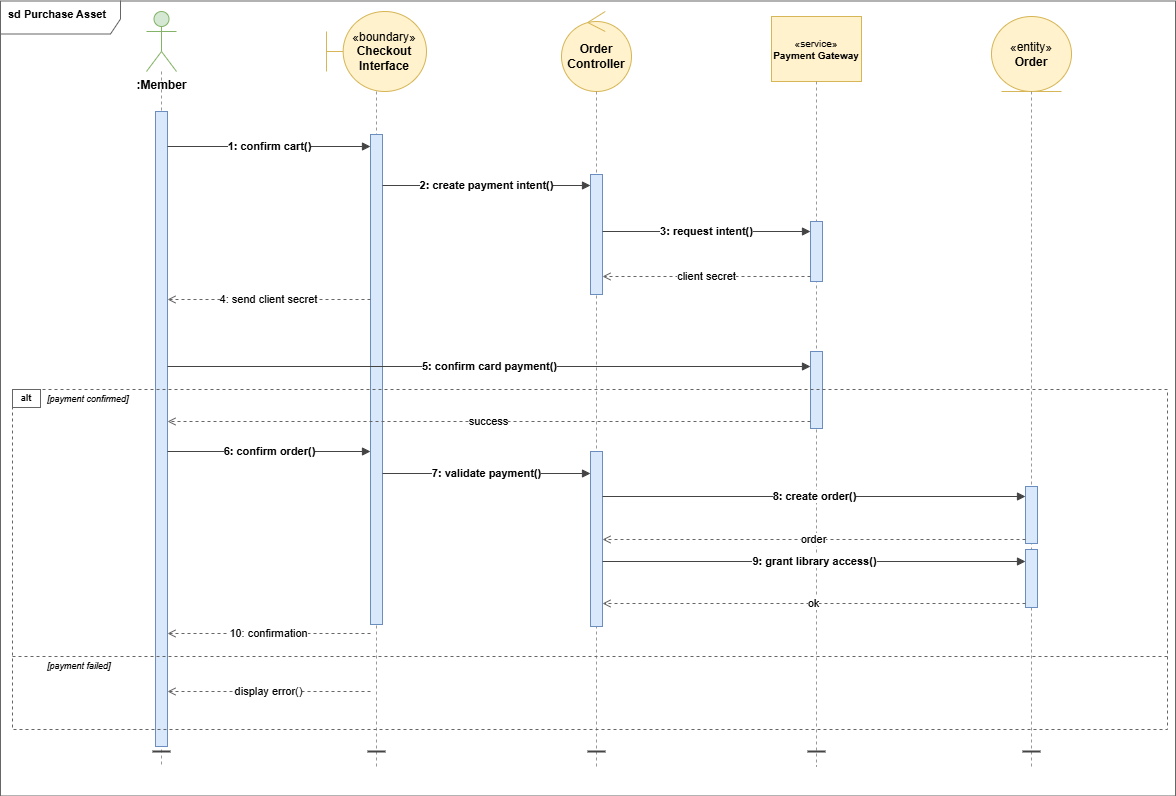
\includegraphics[width=0.95\textwidth]{images/diagrams/seq_payment.png}
\caption{Sequence diagram «Purchase an Asset»}
\label{fig:seq_purchase}
\end{figure}

\paragraph{Sequence diagram «Download from Library».}
When a member clicks Download, the backend re-checks the access level for the asset.
If the access is granted, the backend retrieves the file path and the bucket and
generates a one-hour signed URL through the storage service. The browser uses this
signed URL to fetch the file directly from the CDN, without exposing the bucket path.

\begin{figure}[H]
\centering
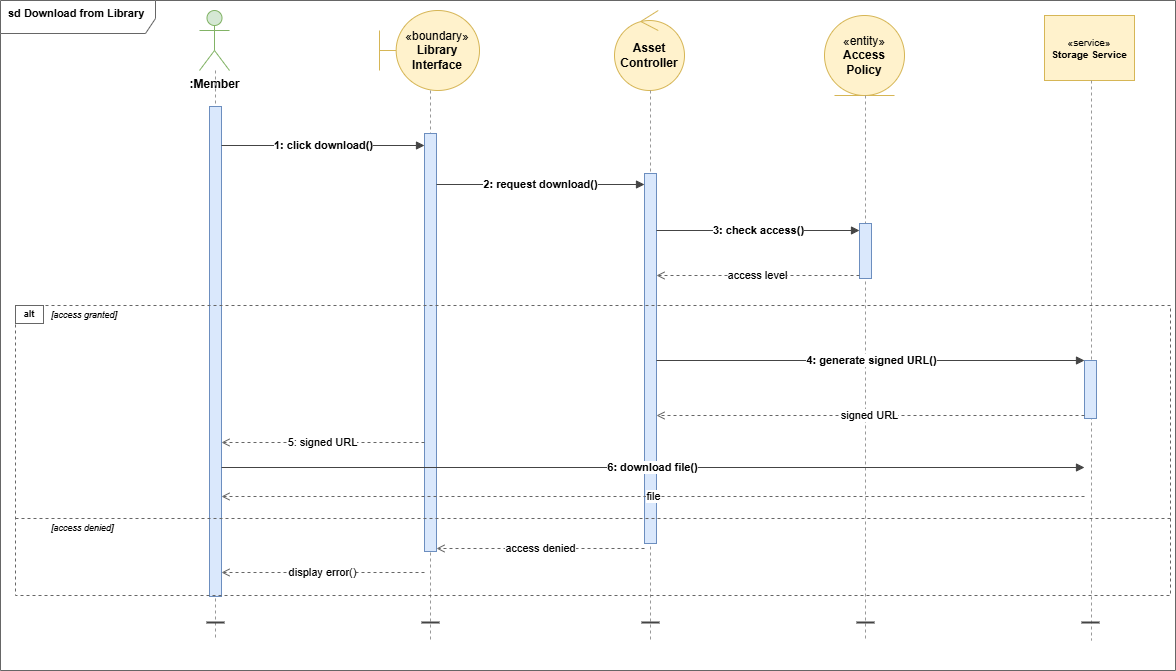
\includegraphics[width=\textwidth]{images/diagrams/seq_download.png}
\caption{Sequence diagram «Download from Library»}
\label{fig:seq_download}
\end{figure}

\subsubsection{Class Diagram}

The class diagram of Sprint~2 introduces the \texttt{Asset} and \texttt{Category}
entities alongside the purchase pipeline: \texttt{CartItem}, \texttt{Order},
\texttt{OrderItem} and \texttt{UserDownload}. Each order item locks the price and
commission split at purchase time so revenue figures remain stable.

\begin{figure}[H]
\centering
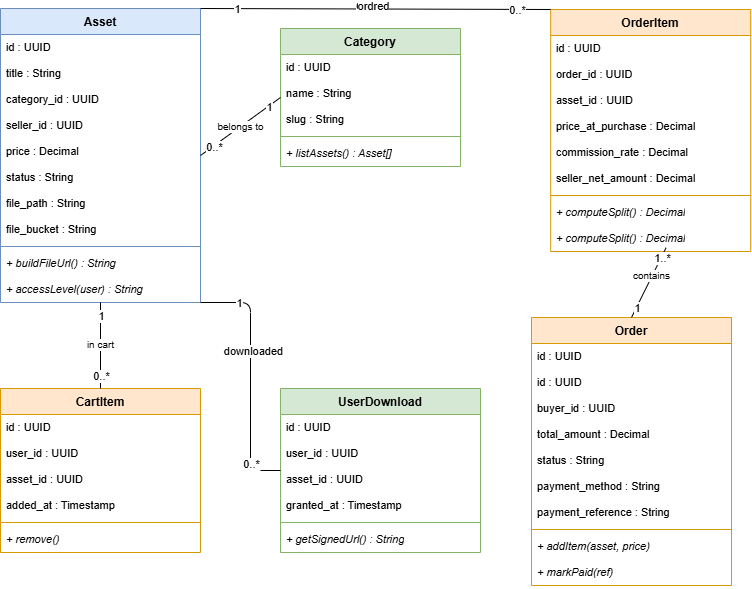
\includegraphics[width=0.95\textwidth]{images/diagrams/class_s2.png}
\caption{Class diagram --- Sprint 2}
\label{fig:class_s2}
\end{figure}

\subsection{Sprint 2 Realization}

In this section we present the interfaces developed during Sprint~2.

\paragraph{«Catalog page».}
This interface lets visitors browse one of the thirteen asset categories. A sidebar
exposes filters by price, rating, tags and file format. Each card shows the
thumbnail, the seller, the price and an interactive preview adapted to the asset
type.

\begin{figure}[H]
\centering
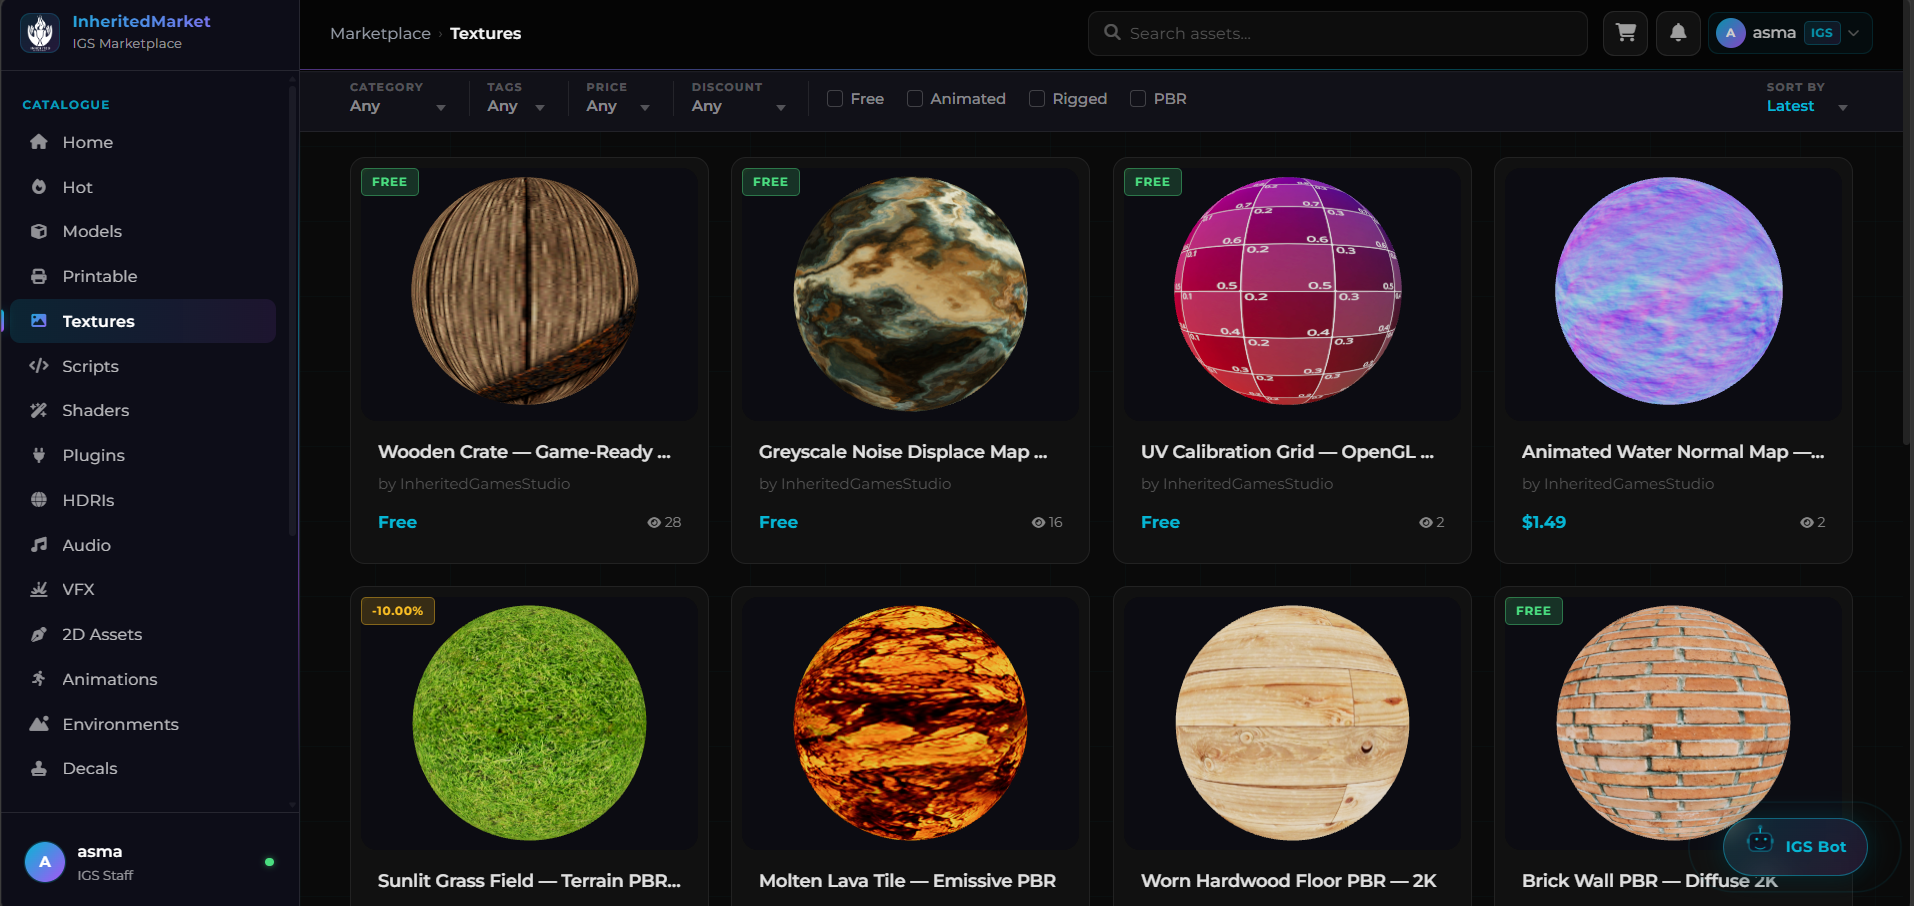
\includegraphics[width=0.85\textwidth]{images/realisation/marketplace/textures page.png}
\caption{Interface «Catalog»}
\end{figure}

\paragraph{«Catalog filters».}
The filter sidebar lets visitors narrow results by price range, rating, tags and file
format. Selections update the catalog grid instantly without a page reload.

\begin{figure}[H]
\centering
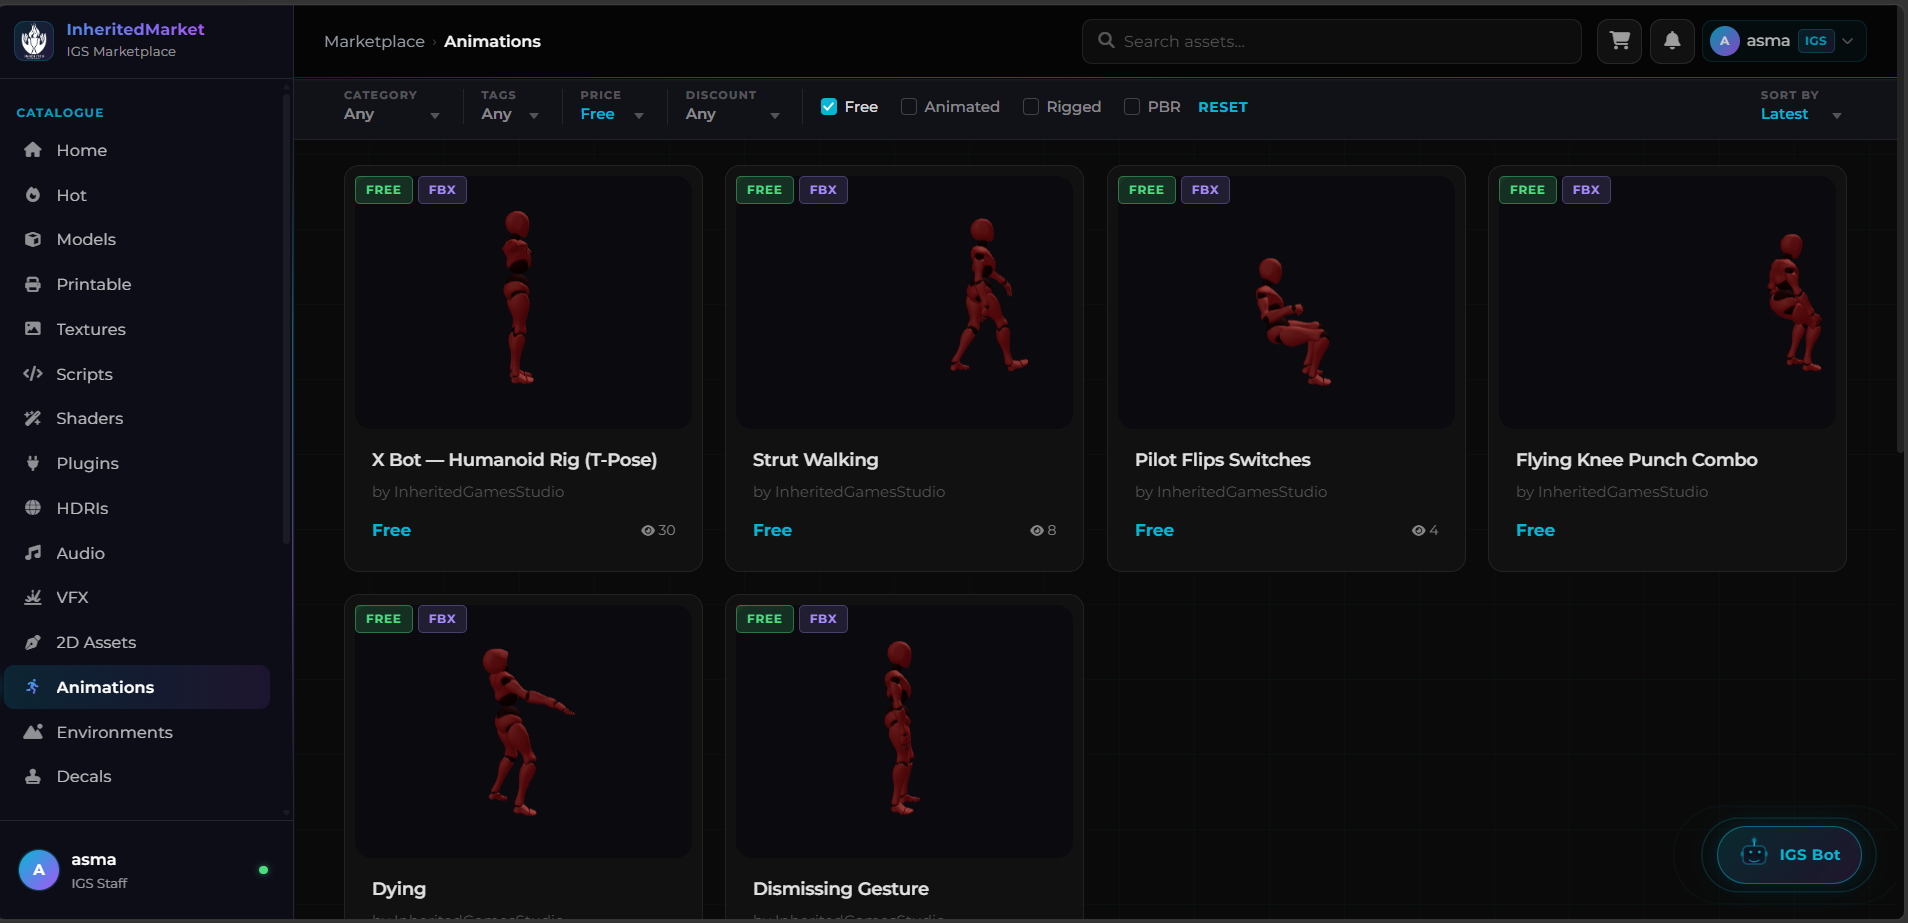
\includegraphics[width=0.85\textwidth]{images/realisation/marketplace/filter.png}
\caption{Interface «Catalog filters»}
\end{figure}

\paragraph{«Shopping cart».}
This interface lists the assets selected by the member. The user can remove an item
or update the quantity, then proceed to checkout with Stripe or Flouci.

\begin{figure}[H]
\centering
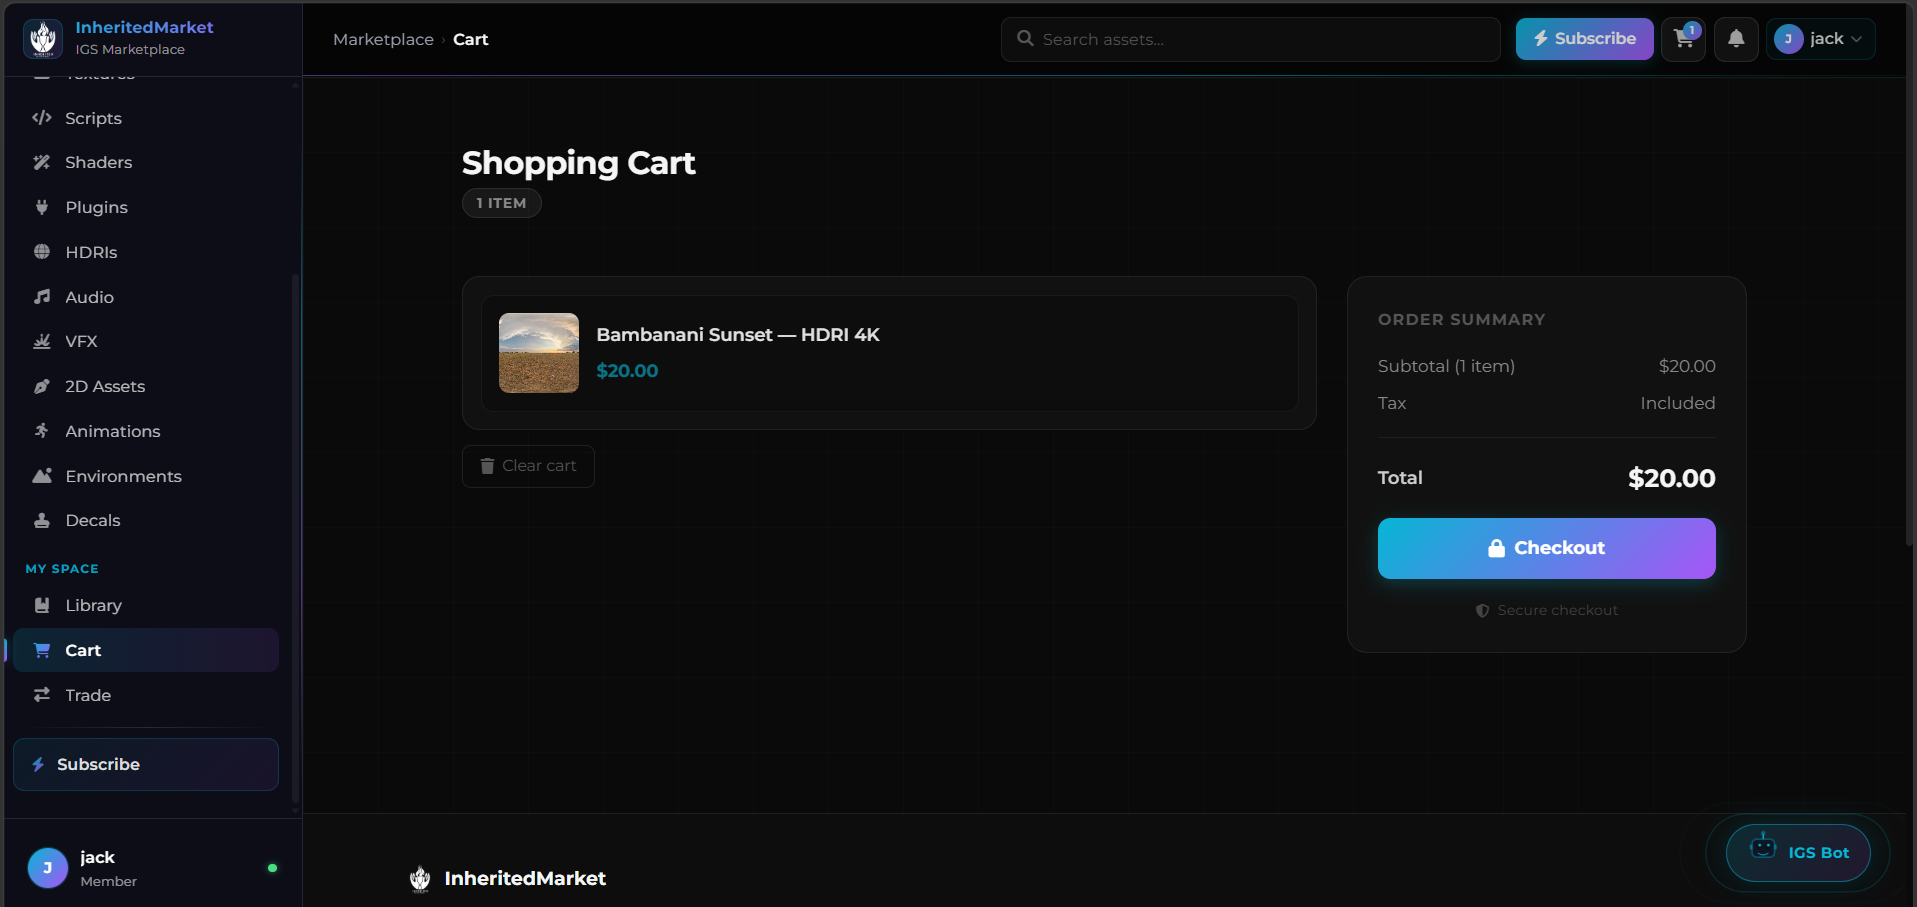
\includegraphics[width=0.85\textwidth]{images/realisation/marketplace/cart.png}
\caption{Interface «Cart»}
\end{figure}

\paragraph{«Library».}
This interface gathers all the assets the member has unlocked (purchased, gifted,
voucher-redeemed or granted by IGS). Each row exposes a Download button that
requests a one-hour signed URL from the backend.

\begin{figure}[H]
\centering
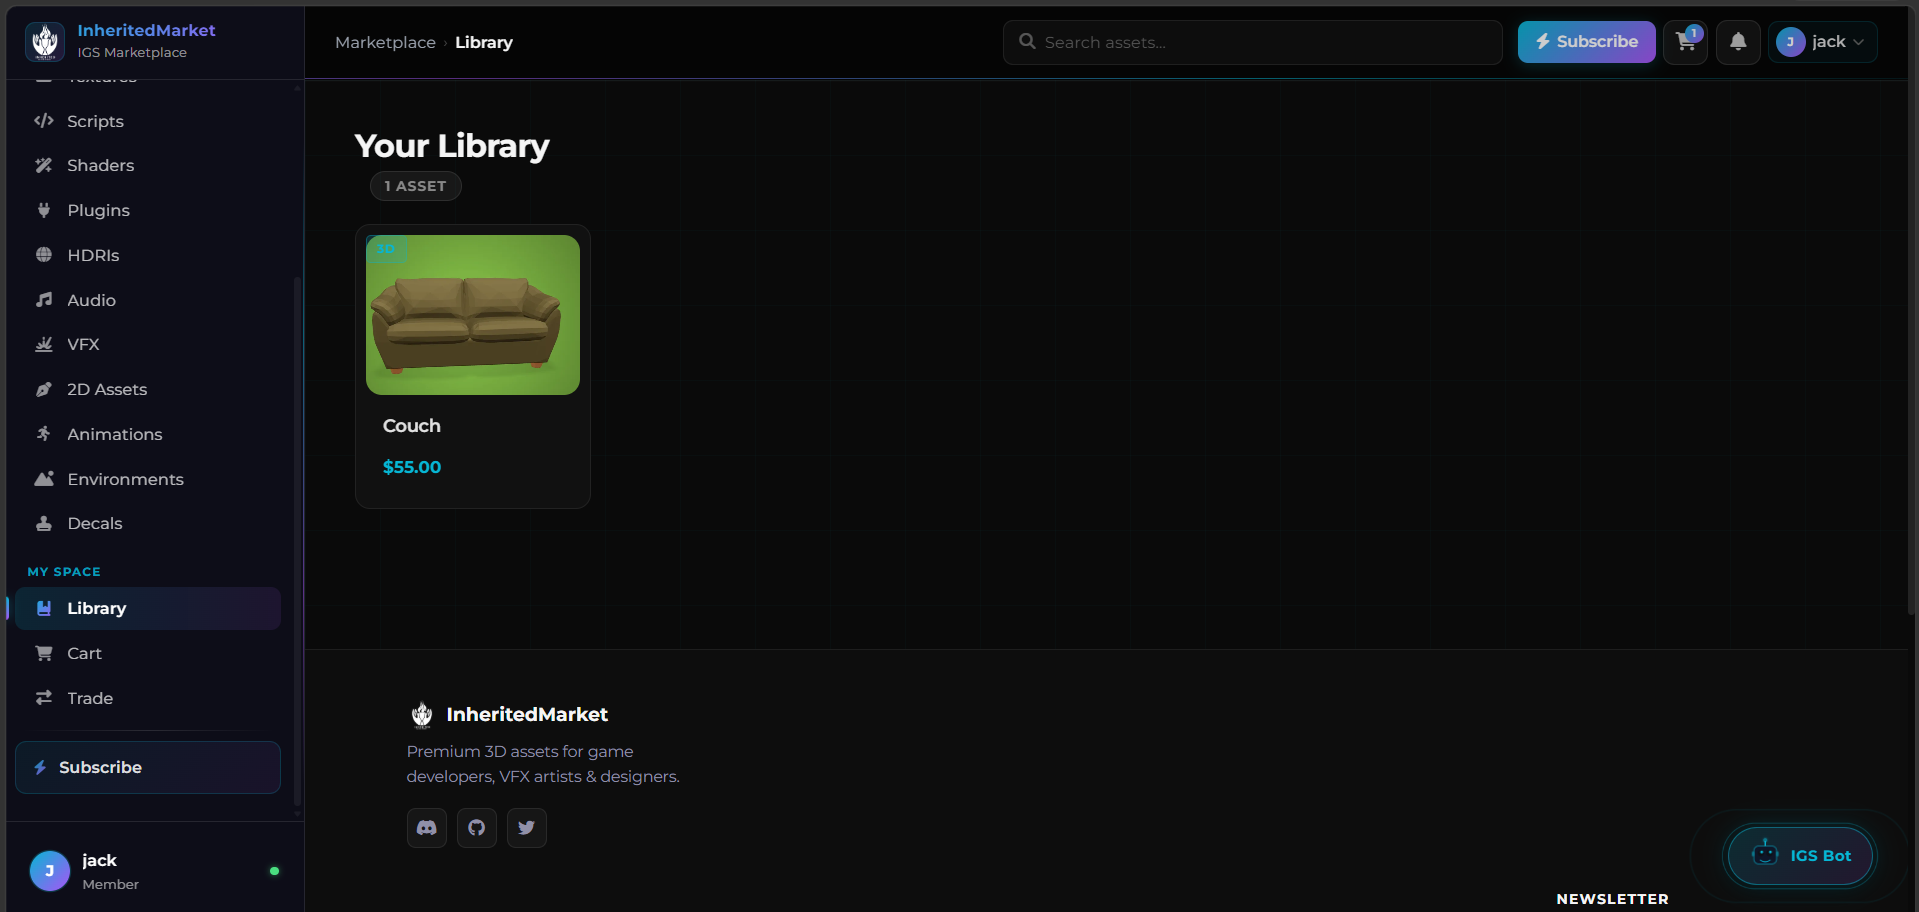
\includegraphics[width=0.85\textwidth]{images/realisation/marketplace/library.png}
\caption{Interface «Library»}
\end{figure}

\subsection{Sprint 2 Conclusion}
At the end of Sprint~2 the public marketplace is fully functional. Visitors can
browse and preview assets in 3D, members can purchase through Stripe or Flouci, and
the personal library exposes time-limited signed downloads.

\section*{Conclusion}
This chapter covered the authentication foundation and the public marketplace implementation across the first two sprints. The following chapter presents Sprint~3 and Sprint~4.

% ============================================================
% CHAPTER 4 — WORKSPACE
% ============================================================
\chapter{Workspace}
\chaptersommaire
\clearpage

\section*{Introduction}
This chapter covers the internal studio workspace and administrative environment that
complement the public marketplace. It explains how the internal application integrates with
the same backend and identity system, and how the workspace was completed with
management dashboards and collaboration tools.

\section{Sprint 5: IGS Workspace}

\subsection{Sprint Backlog}

\begin{sprintbox}{Sprint 5 -- Internal Collaboration Workspace}
\textbf{Goal:} provide IGS employees and interns with an internal workspace connected to
the same authentication and permission system as the marketplace.
\end{sprintbox}

\begin{table}[H]
\centering
\caption{Sprint 5 Backlog}
\begin{tabularx}{\textwidth}{C{1.1cm} X C{2cm}}
\toprule
\textbf{ID} & \textbf{User Story} & \textbf{Priority} \\
\midrule
US-24 & As an internal user, I can access a dedicated workspace dashboard. & High \\
US-25 & As a manager, I can manage team members and positions. & High \\
US-26 & As an internal user, I can create and follow tasks. & High \\
US-27 & As an internal user, I can create projects and assign members. & High \\
US-28 & As a project member, I can attach project documents and view progress. & Medium \\
US-29 & As an internal user, I can chat through channels and direct messages. & Medium \\
\bottomrule
\end{tabularx}
\end{table}

The IGS Workspace was built as a separate React + Vite application under
\texttt{IGS\_Workspace}. It shares the backend API, authentication, and permissions with
the marketplace while providing a distinct internal UI and workflow. Workspace data
includes projects, tasks, team members, project documents, and real-time chat.

\section{Sprint 7: Workspace Completion \& Admin Dashboard}

\subsection{Sprint Backlog}

\begin{sprintbox}{Sprint 7 -- Workspace Completion and Administration}
\textbf{Goal:} complete workspace features and deliver a consolidated administration
experience for internal roles.
\end{sprintbox}

\begin{table}[H]
\centering
\caption{Sprint 7 Backlog}
\begin{tabularx}{\textwidth}{C{1.1cm} X C{2cm}}
\toprule
\textbf{ID} & \textbf{User Story} & \textbf{Priority} \\
\midrule
US-40 & As an administrator, I want a consolidated dashboard with key platform KPIs. & High \\
US-41 & As an internal user, I want placeholder workspace pages replaced with functional content. & Medium \\
US-42 & As an employee, I want workspace reports and calendar features. & Medium \\
US-43 & As an internal user, I want role and permission management inside the workspace. & Medium \\
\bottomrule
\end{tabularx}
\end{table}

Sprint 7 completed the remaining workspace and admin functionality. It polished the internal
navigation, finished the workspace pages for projects, tasks, team, chat, orders, and
reports, and consolidated analytics into a dashboard suitable for managers and supervisors.

\section*{Conclusion}
Chapter 4 demonstrates how IGS Marketplace extends into a private studio environment.
The Workspace chapter describes the internal collaboration tools, team and task management,
chat integration, and final administrative consolidation that make the platform suitable for
both public users and internal staff.

% ============================================================
% CHAPTER 5 — ADVANCED FEATURES
% ============================================================
\chapter{Advanced Features}
\chaptersommaire
\clearpage

\section*{Introduction}
This chapter presents the advanced capabilities that enhance the IGS platform beyond the
basic marketplace and workspace. It covers AI services, recommendation systems,
conversational assistance, premium design, and the deployment pipeline that supports
production delivery.

\section{Sprint 6: AI Services}

\subsection{Sprint Backlog}

\begin{sprintbox}{Sprint 6 -- AI Assistance}
\textbf{Goal:} enrich the platform with AI-supported analysis, recommendations, and
conversational assistance.
\end{sprintbox}

\begin{table}[H]
\centering
\caption{Sprint 6 Backlog}
\begin{tabularx}{\textwidth}{C{1.1cm} X C{2cm}}
\toprule
\textbf{ID} & \textbf{User Story} & \textbf{Priority} \\
\midrule
US-30 & As an admin, I can view AI sentiment information for reviews. & Medium \\
US-31 & As a user, I can receive personalized recommendations. & Medium \\
US-32 & As a visitor or member, I can ask marketplace questions through a chatbot. & Medium \\
US-33 & As the system, I can record user events for recommendation input. & Medium \\
\bottomrule
\end{tabularx}
\end{table}

The AI layer is implemented as a service layer to keep business logic separate from the
API routes. Review sentiment analysis, recommendations, and chatbot intent classification
are all provided through dedicated services, allowing the platform to evolve the AI provider
without changing the core marketplace logic.

\section{Sprint 8: Premium UI \& Platform Delivery}

\subsection{Sprint Backlog}

\begin{sprintbox}{Sprint 8 -- Final Polish and Release Readiness}
\textbf{Goal:} deliver a premium visual experience, complete remaining features, and
prepare the platform for production deployment.
\end{sprintbox}

\begin{table}[H]
\centering
\caption{Sprint 8 Backlog}
\begin{tabularx}{\textwidth}{C{1cm} X C{2cm} C{2.5cm}}
\toprule
\textbf{ID} & \textbf{User Story} & \textbf{Priority} & \textbf{Status} \\
\midrule
US-53 & As an admin, I want a consolidated dashboard with key platform KPIs. & High & \textcolor{igsGreen}{\textbf{Done}} \\
US-54 & As a user, I want the marketplace to have a premium, professional visual identity. & High & \textcolor{igsGreen}{\textbf{Done}} \\
US-55 & As a user, I want a real-time notification panel accessible from any page. & Medium & \textcolor{igsGreen}{\textbf{Done}} \\
US-56 & As any user, I want all placeholder workspace pages to display meaningful content. & Medium & \textcolor{igsGreen}{\textbf{Done}} \\
\bottomrule
\end{tabularx}
\end{table}

This sprint brought the final production polish. The marketplace UI was refined with
consistent branding, improved typography, hover effects, and a premium presentation layer.
The admin dashboard was consolidated around KPI cards and activity feeds, and final
workspace pages were completed to ensure the platform was demonstration-ready.

\section{CI/CD \& Deployment}

\subsection{CI/CD Pipeline}

The deployment pipeline uses GitHub Actions to automate build, test, and production delivery.
A single workflow runs linting, builds, and tests on every push or pull request targeting
\texttt{main}. On successful main branch runs, Docker images are built and pushed, and the
production server is updated via SSH.

\subsection{Containerization and Infrastructure}

Docker is used to package the backend, frontend, and database into reproducible images.
The backend is built from a Node 20 image, the frontend uses a multi-stage Vite build, and
PostgreSQL runs in a managed container with persistent storage. Nginx serves the frontend
bundle and proxies API requests to the Express backend.

\subsection{Deployment Strategy}

The workflow authenticates to DockerHub and the production server using GitHub Secrets.
After pushing images, the deployment job pulls the latest containers and restarts the
stack with minimal manual intervention. Environment variables remain external to the
repository to protect credentials.

\section*{Conclusion}
Chapter 5 highlights the advanced features that give IGS Marketplace a competitive and
professional edge. AI services, premium UI polish, and an automated deployment pipeline
ensure the platform is not only feature-rich but also ready for reliable release and
maintenance.

% ============================================================
% GENERAL CONCLUSION
% ============================================================
\chapter*{General Conclusion}
\addcontentsline{toc}{chapter}{General Conclusion}

IGS Marketplace was successfully designed and developed over five sprints, delivering Tunisia's first dedicated 3D digital asset platform. The system provides a six-level Role-Based Access Control system, an interactive in-browser 3D asset viewer, Stripe payment integration, AI-powered review sentiment analysis, a personalized recommendation engine, a floating chatbot assistant powered by Qwen2.5-72B-Instruct, and a companion internal workspace application — all within a cohesive full-stack ecosystem built on React, Node.js/Express, and PostgreSQL.

Several key technical insights emerged throughout the project. Designing the permission system during Sprint 1 and enforcing it consistently across all subsequent sprints was the single most impactful architectural decision — retrofitting access control would have been significantly more costly. The three-tier layered architecture (Routes → Controllers → Repositories) proved highly maintainable for a REST API at this level of complexity, and applying Scrum as a solo developer, with supervisors occupying the Product Owner and Scrum Master roles, effectively structured six months of work into reviewable, deliverable-focused increments.

Looking ahead, several directions are planned for the platform's continued evolution. The internal workspace application will grow into a full \textbf{ERP system} with richer project management, HR, and operational modules, while its customer-facing side will expand into a comprehensive \textbf{CRM} supporting advanced customer segmentation, relationship tracking, and communication workflows. On the payment front, \textbf{Flouci} integration for Tunisian dinar transactions is already partially in place and will be fully activated once the required administrative and regulatory procedures are completed. The asset catalog will be broadened with new content categories to serve a wider range of creative disciplines. A \textbf{bundle system} will allow sellers to group related assets and offer them at a combined price, increasing average order value and discoverability. Finally, the \textbf{voucher system} — currently scoped to internal users — will be extended to all user types, enabling promotional campaigns for members, sellers, and subscribers alike. These evolutions position the IGS Marketplace as a long-term, scalable platform well beyond its current scope.


% ---- BIBLIOGRAPHY & WEBOGRAPHY (numbered, merged) ----
\clearpage
\renewcommand{\bibname}{Webography}
\addcontentsline{toc}{chapter}{Webography}
\begin{thebibliography}{99}

\bibitem{citius2024}
Citius Research. \textit{3D Project Market Report}. 2024.\\
\url{https://citiusresearch.com/publication-details/3d-project-market-report} \quad [Accessed April 2026]

\bibitem{pmarket2024}
P Market Research. \textit{Worldwide 3D Marketplace Models Market Research 2024 ---
by Type, Application, Participants and Countries, Forecast to 2030}. 2024.\\
\url{https://pmarketresearch.com/worldwide-3d-marketplace-models-market-research-2024-by-type-application-participants-and-countries-forecast-to-2030/} \quad [Accessed April 2026]

\bibitem{unityassetstore}
Unity Technologies. \textit{Unity Asset Store}.\\
\url{https://assetstore.unity.com/} \quad [Accessed April 2026]

\bibitem{epicfab}
Epic Games. \textit{Fab --- The unified content marketplace by Epic Games}.\\
\url{https://www.fab.com/} \quad [Accessed April 2026]

\bibitem{sketchfab}
Sketchfab (Epic Games). \textit{Sketchfab --- Publish \& Find 3D Models Online}.\\
\url{https://sketchfab.com/} \quad [Accessed April 2026]

\bibitem{cgtrader}
CGTrader. \textit{CGTrader --- 3D Model Marketplace and Computer Graphics Forum}.\\
\url{https://www.cgtrader.com/} \quad [Accessed April 2026]

\bibitem{agilethinking}
AgileThinkin.pro. \textit{Qu'est-ce que Scrum ?}.\\
\url{https://agilethinking.pro/quest-ce-que-scrum/} \quad [Accessed May 2026]

\bibitem{metaquest}
Meta Platforms, Inc. \textit{Meta Quest 3 --- Mixed Reality Headset}.\\
\url{https://www.meta.com/quest/quest-3/} \quad [Accessed May 2026]

\bibitem{vscode}
Microsoft. \textit{Visual Studio Code --- Code Editing Redefined}.\\
\url{https://code.visualstudio.com/} \quad [Accessed May 2026]

\bibitem{github}
GitHub, Inc. \textit{GitHub --- Where the world builds software}.\\
\url{https://github.com/} \quad [Accessed May 2026]

\bibitem{hostinger}
Hostinger International. \textit{Hostinger --- Web Hosting and VPS}.\\
\url{https://www.hostinger.com/} \quad [Accessed May 2026]

\bibitem{drawio}
JGraph Ltd. \textit{draw.io --- Free Online Diagram Software}.\\
\url{https://www.drawio.com/} \quad [Accessed May 2026]

\bibitem{eslint}
OpenJS Foundation. \textit{ESLint --- Find and fix problems in JavaScript code}.\\
\url{https://eslint.org/} \quad [Accessed May 2026]

\bibitem{reactdoc}
Meta Platforms. \textit{React --- The library for web and native user interfaces}.\\
\url{https://react.dev/} \quad [Accessed April 2026]

\bibitem{socketio}
Socket.IO contributors. \textit{Socket.IO v4 Documentation}.\\
\url{https://socket.io/docs/v4/} \quad [Accessed April 2026]

\bibitem{expressdoc}
OpenJS Foundation. \textit{Express.js Application Guide}.\\
\url{https://expressjs.com/en/guide/routing.html} \quad [Accessed April 2026]

\bibitem{supabasestorage}
Supabase Inc. \textit{Supabase Documentation --- Storage}.\\
\url{https://supabase.com/docs/guides/storage} \quad [Accessed April 2026]

\bibitem{supabaseauth}
Supabase Inc. \textit{Supabase Documentation --- Auth}.\\
\url{https://supabase.com/docs/guides/auth} \quad [Accessed April 2026]

\bibitem{stripeapi}
Stripe, Inc. \textit{Stripe API Reference --- Payment Intents}.\\
\url{https://stripe.com/docs/api/payment_intents} \quad [Accessed April 2026]

\bibitem{huggingface}
Hugging Face. \textit{Inference API Documentation}.\\
\url{https://huggingface.co/docs/api-inference} \quad [Accessed April 2026]

\bibitem{tfidf}
Salton, G. \& Buckley, C. (1988). Term-weighting approaches in automatic text retrieval.
\textit{Information Processing \& Management}, 24(5), 513--523.

\bibitem{svm}
Cortes, C. \& Vapnik, V. (1995). Support-vector networks.
\textit{Machine Learning}, 20(3), 273--297.

\bibitem{sklearn}
Pedregosa, F. et al. (2011). Scikit-learn: Machine Learning in Python.
\textit{Journal of Machine Learning Research}, 12, 2825--2830.\\
\url{https://scikit-learn.org/} \quad [Accessed May 2026]

\bibitem{rag}
Lewis, P. et al. (2020). Retrieval-Augmented Generation for Knowledge-Intensive NLP Tasks.
\textit{Advances in Neural Information Processing Systems}, 33.\\
\url{https://arxiv.org/abs/2005.11401} \quad [Accessed May 2026]

\bibitem{qwen25}
Qwen Team, Alibaba Cloud. \textit{Qwen2.5: A Party of Foundation Models}. 2024.\\
\url{https://huggingface.co/Qwen/Qwen2.5-72B-Instruct} \quad [Accessed May 2026]

\bibitem{transformer}
Vaswani, A. et al. (2017). Attention Is All You Need.
\textit{Advances in Neural Information Processing Systems}, 30.\\
\url{https://arxiv.org/abs/1706.03762} \quad [Accessed May 2026]

\bibitem{distilbert}
Sanh, V. et al. (2019). DistilBERT, a distilled version of BERT: smaller, faster, cheaper and lighter.\\
\url{https://arxiv.org/abs/1910.01108} \quad [Accessed May 2026]

\bibitem{bert}
Devlin, J. et al. (2018). BERT: Pre-training of Deep Bidirectional Transformers for Language Understanding.\\
\url{https://arxiv.org/abs/1810.04805} \quad [Accessed May 2026]

\bibitem{sst2}
Socher, R. et al. (2013). Recursive Deep Models for Semantic Compositionality Over a Sentiment Treebank.
\textit{Proceedings of EMNLP 2013}.\\
\url{https://nlp.stanford.edu/sentiment/} \quad [Accessed May 2026]

\bibitem{cbf}
Lops, P., de Gemmis, M. \& Semeraro, G. (2011). Content-based Recommender Systems: State of the Art and Trends.
In F. Ricci et al.\ (Eds.), \textit{Recommender Systems Handbook}. Springer.

\bibitem{jaccard}
Jaccard, P. (1912). The distribution of the flora in the alpine zone.
\textit{New Phytologist}, 11(2), 37--50.

\bibitem{owasp}
OWASP Foundation. \textit{OWASP Top Ten --- Web Application Security Risks}.\\
\url{https://owasp.org/www-project-top-ten/} \quad [Accessed April 2026]

\bibitem{webxr}
W3C. \textit{WebXR Device API --- W3C Candidate Recommendation}. 2024.\\
\url{https://www.w3.org/TR/webxr/} \quad [Accessed May 2026]

\bibitem{webgl}
Khronos Group. \textit{WebGL 1.0 Specification}. 2011.\\
\url{https://www.khronos.org/registry/webgl/specs/latest/1.0/} \quad [Accessed May 2026]

\bibitem{threejs}
Three.js contributors. \textit{Three.js --- JavaScript 3D Library}.\\
\url{https://threejs.org/docs/} \quad [Accessed April 2026]

% ---- Supplementary references (not cited inline) ----

\bibitem{cosmosplatform}
Threedy.ai. \textit{Cosmos --- AI-powered 3D content platform}.\\
\url{https://www.threedy.ai/} \quad [Accessed April 2026]

\bibitem{docker}
Docker, Inc. \textit{Docker --- Accelerated Container Application Development}.\\
\url{https://www.docker.com/} \quad [Accessed May 2026]

\bibitem{githubactions}
GitHub, Inc. \textit{GitHub Actions Documentation}.\\
\url{https://docs.github.com/en/actions} \quad [Accessed May 2026]

\bibitem{jwt}
Jones, M. et al. \textit{RFC 7519 --- JSON Web Token (JWT)}. IETF, 2015.\\
\url{https://datatracker.ietf.org/doc/html/rfc7519} \quad [Accessed April 2026]

\bibitem{mixamo}
Adobe Inc. \textit{Mixamo --- Free animated 3D characters}.\\
\url{https://www.mixamo.com/} \quad [Accessed April 2026]

\bibitem{modelviewer}
Google LLC. \textit{Model Viewer --- Web Component for 3D Models}.\\
\url{https://modelviewer.dev/} \quad [Accessed April 2026]

\bibitem{nodedoc}
OpenJS Foundation. \textit{Node.js Official Documentation}.\\
\url{https://nodejs.org/en/docs/} \quad [Accessed April 2026]

\bibitem{pgdoc}
The PostgreSQL Global Development Group. \textit{PostgreSQL 16 Documentation}.\\
\url{https://www.postgresql.org/docs/16/} \quad [Accessed April 2026]

\bibitem{rbac}
Ferraiolo, D. \& Kuhn, R. \textit{Role-Based Access Control}. NIST, 2009.

\bibitem{roques}
Roques, P. \textit{UML 2 par la Pratique --- Études de cas et exercices corrigés}.
8\textsuperscript{e} édition. Eyrolles, 2014.

\bibitem{scrum}
Schwaber, K. \& Sutherland, J. \textit{The Scrum Guide}. November 2020.\\
\url{https://scrumguides.org/scrum-guide.html} \quad [Accessed April 2026]

\bibitem{tailwindcss}
Tailwind Labs. \textit{Tailwind CSS --- A utility-first CSS framework}.\\
\url{https://tailwindcss.com/} \quad [Accessed May 2026]

\bibitem{toollogos}
Tool logos used throughout this report were obtained from the official websites
of the respective projects: React, Node.js, Express, Vite, PostgreSQL, Supabase,
Stripe, Socket.IO, Three.js, Hugging Face, Docker, GitHub, GitHub Actions,
draw.io, ESLint, Tailwind CSS, JWT, Hostinger, Meta Quest and \LaTeX.\\
\url{https://react.dev/} ; \url{https://nodejs.org/} ; \url{https://threejs.org/}
\quad [Accessed May 2026]

\bibitem{uml}
Object Management Group. \textit{UML 2.5.1 Specification}. 2017.\\
\url{https://www.omg.org/spec/UML/2.5.1} \quad [Accessed April 2026]

\bibitem{vitedoc}
Vite contributors. \textit{Vite --- Next generation frontend tooling}.\\
\url{https://vitejs.dev/guide/} \quad [Accessed April 2026]

\end{thebibliography}

% ---- ABSTRACT (last page) ----
\clearpage
% ============================================================
% ABSTRACT -- single page, three languages
% ============================================================
\thispagestyle{empty}
\newgeometry{top=1.6cm, bottom=1.6cm, left=2.2cm, right=2.2cm}
\addcontentsline{toc}{chapter}{Abstract}

\noindent\rule{\textwidth}{1.5pt}

% ---- English ----
\vspace{0.1cm}
\begin{center}{\bfseries\large\color{isiBlue} Abstract}\end{center}
\vspace{0.05cm}
\footnotesize
\setlength{\parskip}{4pt}

This end-of-studies project presents the design and development of \textbf{IGS Marketplace},
a full-stack digital platform built for \textbf{Inherited Games Studio (IGS)}, a Tunisian
video-game company. The solution addresses the absence of a national marketplace for
3D creative content by offering local creators a dedicated space to publish and monetize
their work, with secure payments in both international and Tunisian currency.

The platform consists of two complementary applications sharing a common back-end: a
public \textit{Marketplace} covering thirteen asset categories with interactive 3D and
WebXR previews on virtual-reality headsets, and an internal \textit{Workspace} for
project management, content moderation and administration. Three AI services are
integrated --- a conversational chatbot, a DistilBERT-based review sentiment analyzer
and a Jaccard-based recommendation engine. The technical stack relies on \textbf{React},
\textbf{Node.js / Express} and \textbf{PostgreSQL (Supabase)}, following the \textbf{Scrum}
methodology over five sprints.\\[1pt]
\textbf{Keywords:} 3D Marketplace, WebXR, React, Node.js, PostgreSQL, RBAC, Scrum, Artificial Intelligence.

\noindent\rule{\textwidth}{0.4pt}

% ---- French ----
\vspace{0.1cm}
\begin{center}{\bfseries\large\color{isiBlue} Résumé}\end{center}
\vspace{0.05cm}
\footnotesize

Ce projet de fin d'études présente la conception et le développement de
\textbf{IGS Marketplace}, une plateforme web full-stack réalisée pour
\textbf{Inherited Games Studio (IGS)}, société tunisienne de développement de jeux vidéo.
La solution répond à l'absence d'une marketplace nationale dédiée aux contenus 3D, en
offrant aux créateurs locaux un espace de publication et de monétisation avec un
paiement sécurisé en devises internationales et en dinar.

La plateforme se compose de deux applications partageant un back-end commun: une
\textit{Marketplace} publique couvrant treize catégories d'assets avec prévisualisation
3D interactive et mode immersif WebXR sur casques de réalité virtuelle, et un
\textit{Workspace} interne pour la gestion de projet, la modération et l'administration.
Trois services d'intelligence artificielle sont intégrés --- un chatbot conversationnel,
une analyse de sentiment basée sur DistilBERT et un moteur de recommandations
reposant sur la similarité de Jaccard. La pile technique repose sur \textbf{React},
\textbf{Node.js / Express} et \textbf{PostgreSQL (Supabase)}, suivant la méthodologie
\textbf{Scrum} sur cinq sprints.\\[1pt]
\textbf{Mots-clés :} Marketplace 3D, WebXR, React, Node.js, PostgreSQL, RBAC, Scrum, Intelligence Artificielle.

\noindent\rule{\textwidth}{0.4pt}

% ---- Arabic ----
\begin{Arabic}
\vspace{0.1cm}
\begin{center}{\bfseries\large\color{isiBlue} ملخص}\end{center}
\vspace{0.05cm}
\footnotesize

يقدم هذا المشروع تصميم وتطوير منصة \textbf{IGS Marketplace} لفائدة شركة
\textbf{Inherited Games Studio} التونسية المتخصصة في تطوير ألعاب الفيديو. تعالج
المنصة غياب فضاء وطني مخصص للأصول الإبداعية ثلاثية الأبعاد، وتوفر للمبدعين المحليين
فضاءً للنشر والبيع مع دعم الدفع الآمن بالعملات الدولية وبالدينار التونسي.

تتكون المنصة من تطبيقين متكاملين يشتركان في خادم خلفي موحد: واجهة عامة
\textit{Marketplace} تغطي ثلاث عشرة فئة من الأصول الرقمية مع عرض تفاعلي ومعاينة
غامرة عبر تقنية WebXR، ولوحة تحكم داخلية \textit{Workspace} لإدارة المشاريع
ومراقبة المحتوى. تدمج المنصة ثلاث خدمات للذكاء الاصطناعي: روبوت محادثة، ومحلل
لمشاعر التقييمات يعتمد على نموذج DistilBERT، ومحرك توصيات مبني على مقياس Jaccard.
وتعتمد التقنيات المستخدمة على \textbf{React} و\textbf{Node.js / Express}
و\textbf{PostgreSQL (Supabase)}، باتباع منهجية \textbf{Scrum} عبر خمس دورات تطويرية.\\[1pt]
\textbf{الكلمات المفتاحية:} منصة ثلاثية الأبعاد، WebXR، React، Node.js، PostgreSQL، RBAC، Scrum، ذكاء اصطناعي.
\end{Arabic}

\noindent\rule{\textwidth}{1.5pt}

\restoregeometry


\end{document}
